\documentclass[11pt]{article}

% ============================================================
%  BBCN preprint scaffold (LaTeX)
%  Working scaffold: every number/figure/table is fixed and
%  reproducible from the companion repository (reproduce_all.py).
%  Final prose to be authored separately.
% ============================================================

\usepackage[utf8]{inputenc}
\usepackage[T1]{fontenc}
% \usepackage{lmodern} % optional; uncomment if installed
\usepackage[margin=1in]{geometry}
\usepackage{graphicx}
\graphicspath{{./}{figures/}}
\usepackage{amsmath,amssymb}
\usepackage{booktabs}
\usepackage{authblk}
\usepackage{xcolor}
\usepackage{caption}
\usepackage{float}
\usepackage[hidelinks]{hyperref}
\usepackage{xurl}
\captionsetup{font=small,labelfont=bf}

\definecolor{navy}{HTML}{1F3864}
\definecolor{authornote}{HTML}{9C6500}
\newcommand{\authornote}[1]{\par\noindent{\small\itshape\color{authornote}[Author note: #1]}\par}
% Internal to-dos: kept in source but suppressed in the posted/submitted build.
\renewcommand{\authornote}[1]{}

\title{\textbf{The Boolean Breast-Cancer Network (BBCN): durable, controllable apoptosis from faithful feedback and multi-timescale control}}
\author[1]{Aamer Iqbal Bhatti\thanks{Corresponding author. ORCID: 0000-0002-3373-3388.}}
\affil[1]{Department of Control and Instrumentation Engineering, King Fahd University of Petroleum and Minerals, Dhahran, Saudi Arabia}
\date{June 2026}

% All numerical values below come from results/numbers/numbers.tex, auto-generated
% by run_chunked.py over the full cohorts. The preprint never hard-codes a number.
% AUTO-GENERATED by run_chunked.py --emit — DO NOT EDIT BY HAND.
\newcommand{\BBCNACdeRankedIspyTwoStagepassApoptosisOn}{39}
\newcommand{\BBCNACdeRankedIspyTwoStagepassProliferationOff}{60}
\newcommand{\BBCNACdeRankedIspyTwoStagepassResistanceOff}{13}
\newcommand{\BBCNACdeRankedIspyTwoStagepassTerminal}{4}
\newcommand{\BBCNACdeRankedMetabricStagepassApoptosisOn}{33}
\newcommand{\BBCNACdeRankedMetabricStagepassProliferationOff}{61}
\newcommand{\BBCNACdeRankedMetabricStagepassResistanceOff}{7}
\newcommand{\BBCNACdeRankedMetabricStagepassTerminal}{1}
\newcommand{\BBCNACdeRankedTcgaStagepassApoptosisOn}{31}
\newcommand{\BBCNACdeRankedTcgaStagepassProliferationOff}{65}
\newcommand{\BBCNACdeRankedTcgaStagepassResistanceOff}{14}
\newcommand{\BBCNACdeRankedTcgaStagepassTerminal}{4}
\newcommand{\BBCNACdeStabilizeIspyTwoStagepassApoptosisOn}{35}
\newcommand{\BBCNACdeStabilizeIspyTwoStagepassProliferationOff}{43}
\newcommand{\BBCNACdeStabilizeIspyTwoStagepassResistanceOff}{8}
\newcommand{\BBCNACdeStabilizeIspyTwoStagepassTerminal}{3}
\newcommand{\BBCNACdeStabilizeMetabricStagepassApoptosisOn}{29}
\newcommand{\BBCNACdeStabilizeMetabricStagepassProliferationOff}{40}
\newcommand{\BBCNACdeStabilizeMetabricStagepassResistanceOff}{4}
\newcommand{\BBCNACdeStabilizeMetabricStagepassTerminal}{1}
\newcommand{\BBCNACdeStabilizeTcgaStagepassApoptosisOn}{27}
\newcommand{\BBCNACdeStabilizeTcgaStagepassProliferationOff}{39}
\newcommand{\BBCNACdeStabilizeTcgaStagepassResistanceOff}{8}
\newcommand{\BBCNACdeStabilizeTcgaStagepassTerminal}{3}
\newcommand{\BBCNAStaticRankedIspyTwoIsoApoptosisOn}{81}
\newcommand{\BBCNAStaticRankedIspyTwoIsoProliferationOff}{94}
\newcommand{\BBCNAStaticRankedIspyTwoIsoResistanceOff}{8}
\newcommand{\BBCNAStaticRankedIspyTwoN}{988}
\newcommand{\BBCNAStaticRankedIspyTwoSeqAllThree}{3}
\newcommand{\BBCNAStaticRankedIspyTwoSeqApoptosisOn}{9}
\newcommand{\BBCNAStaticRankedIspyTwoSeqProliferationOff}{4}
\newcommand{\BBCNAStaticRankedIspyTwoSeqResistanceOff}{8}
\newcommand{\BBCNAStaticRankedMetabricIsoApoptosisOn}{85}
\newcommand{\BBCNAStaticRankedMetabricIsoProliferationOff}{95}
\newcommand{\BBCNAStaticRankedMetabricIsoResistanceOff}{4}
\newcommand{\BBCNAStaticRankedMetabricN}{1980}
\newcommand{\BBCNAStaticRankedMetabricSeqAllThree}{2}
\newcommand{\BBCNAStaticRankedMetabricSeqApoptosisOn}{5}
\newcommand{\BBCNAStaticRankedMetabricSeqProliferationOff}{2}
\newcommand{\BBCNAStaticRankedMetabricSeqResistanceOff}{4}
\newcommand{\BBCNAStaticRankedTcgaIsoApoptosisOn}{86}
\newcommand{\BBCNAStaticRankedTcgaIsoProliferationOff}{94}
\newcommand{\BBCNAStaticRankedTcgaIsoResistanceOff}{8}
\newcommand{\BBCNAStaticRankedTcgaN}{1082}
\newcommand{\BBCNAStaticRankedTcgaSeqAllThree}{3}
\newcommand{\BBCNAStaticRankedTcgaSeqApoptosisOn}{9}
\newcommand{\BBCNAStaticRankedTcgaSeqProliferationOff}{3}
\newcommand{\BBCNAStaticRankedTcgaSeqResistanceOff}{8}
\newcommand{\BBCNAStaticStabilizeIspyTwoIsoApoptosisOn}{87}
\newcommand{\BBCNAStaticStabilizeIspyTwoIsoProliferationOff}{91}
\newcommand{\BBCNAStaticStabilizeIspyTwoIsoResistanceOff}{5}
\newcommand{\BBCNAStaticStabilizeIspyTwoN}{988}
\newcommand{\BBCNAStaticStabilizeIspyTwoSeqAllThree}{2}
\newcommand{\BBCNAStaticStabilizeIspyTwoSeqApoptosisOn}{12}
\newcommand{\BBCNAStaticStabilizeIspyTwoSeqProliferationOff}{2}
\newcommand{\BBCNAStaticStabilizeIspyTwoSeqResistanceOff}{5}
\newcommand{\BBCNAStaticStabilizeMetabricIsoApoptosisOn}{89}
\newcommand{\BBCNAStaticStabilizeMetabricIsoProliferationOff}{91}
\newcommand{\BBCNAStaticStabilizeMetabricIsoResistanceOff}{3}
\newcommand{\BBCNAStaticStabilizeMetabricN}{1980}
\newcommand{\BBCNAStaticStabilizeMetabricSeqAllThree}{1}
\newcommand{\BBCNAStaticStabilizeMetabricSeqApoptosisOn}{6}
\newcommand{\BBCNAStaticStabilizeMetabricSeqProliferationOff}{1}
\newcommand{\BBCNAStaticStabilizeMetabricSeqResistanceOff}{3}
\newcommand{\BBCNAStaticStabilizeTcgaIsoApoptosisOn}{91}
\newcommand{\BBCNAStaticStabilizeTcgaIsoProliferationOff}{85}
\newcommand{\BBCNAStaticStabilizeTcgaIsoResistanceOff}{5}
\newcommand{\BBCNAStaticStabilizeTcgaN}{1082}
\newcommand{\BBCNAStaticStabilizeTcgaSeqAllThree}{2}
\newcommand{\BBCNAStaticStabilizeTcgaSeqApoptosisOn}{11}
\newcommand{\BBCNAStaticStabilizeTcgaSeqProliferationOff}{2}
\newcommand{\BBCNAStaticStabilizeTcgaSeqResistanceOff}{5}
\newcommand{\BBCNBKernelRankedIspyTwoFlipPct}{46}
\newcommand{\BBCNBKernelRankedIspyTwoKerDesigned}{430}
\newcommand{\BBCNBKernelRankedIspyTwoKerSuccess}{198}
\newcommand{\BBCNBKernelRankedIspyTwoTopNode}{PIK3CA}
\newcommand{\BBCNBKernelRankedMetabricFlipPct}{42}
\newcommand{\BBCNBKernelRankedMetabricKerDesigned}{890}
\newcommand{\BBCNBKernelRankedMetabricKerSuccess}{373}
\newcommand{\BBCNBKernelRankedMetabricTopNode}{PIK3CA}
\newcommand{\BBCNBKernelRankedTcgaFlipPct}{47}
\newcommand{\BBCNBKernelRankedTcgaKerDesigned}{428}
\newcommand{\BBCNBKernelRankedTcgaKerSuccess}{202}
\newcommand{\BBCNBKernelRankedTcgaTopNode}{PIK3CA}
\newcommand{\BBCNBKernelStabilizeIspyTwoFlipPct}{46}
\newcommand{\BBCNBKernelStabilizeIspyTwoKerDesigned}{430}
\newcommand{\BBCNBKernelStabilizeIspyTwoKerSuccess}{198}
\newcommand{\BBCNBKernelStabilizeIspyTwoTopNode}{PIK3CA}
\newcommand{\BBCNBKernelStabilizeMetabricFlipPct}{42}
\newcommand{\BBCNBKernelStabilizeMetabricKerDesigned}{890}
\newcommand{\BBCNBKernelStabilizeMetabricKerSuccess}{373}
\newcommand{\BBCNBKernelStabilizeMetabricTopNode}{PIK3CA}
\newcommand{\BBCNBKernelStabilizeTcgaFlipPct}{47}
\newcommand{\BBCNBKernelStabilizeTcgaKerDesigned}{428}
\newcommand{\BBCNBKernelStabilizeTcgaKerSuccess}{202}
\newcommand{\BBCNBKernelStabilizeTcgaTopNode}{PIK3CA}
\newcommand{\BBCNBRoutingSwitchIspyTwoApopPct}{51}
\newcommand{\BBCNBRoutingSwitchIspyTwoMixedPct}{23}
\newcommand{\BBCNBRoutingSwitchIspyTwoN}{988}
\newcommand{\BBCNBRoutingSwitchIspyTwoResistApopZ}{0.08}
\newcommand{\BBCNBRoutingSwitchIspyTwoResistSurvZ}{0.32}
\newcommand{\BBCNBRoutingSwitchIspyTwoSurvPct}{25}
\newcommand{\BBCNBRoutingSwitchIspyTwoSurvUncoupledPct}{89}
\newcommand{\BBCNBRoutingSwitchIspyTwoUPct}{26}
\newcommand{\BBCNBRoutingSwitchMetabricApopPct}{48}
\newcommand{\BBCNBRoutingSwitchMetabricMixedPct}{22}
\newcommand{\BBCNBRoutingSwitchMetabricN}{1980}
\newcommand{\BBCNBRoutingSwitchMetabricResistApopZ}{0.11}
\newcommand{\BBCNBRoutingSwitchMetabricResistSurvZ}{0.2}
\newcommand{\BBCNBRoutingSwitchMetabricSurvPct}{29}
\newcommand{\BBCNBRoutingSwitchMetabricSurvUncoupledPct}{90}
\newcommand{\BBCNBRoutingSwitchMetabricUPct}{29}
\newcommand{\BBCNBRoutingSwitchTcgaApopPct}{50}
\newcommand{\BBCNBRoutingSwitchTcgaMixedPct}{14}
\newcommand{\BBCNBRoutingSwitchTcgaN}{1082}
\newcommand{\BBCNBRoutingSwitchTcgaResistApopZ}{0.32}
\newcommand{\BBCNBRoutingSwitchTcgaResistSurvZ}{0.8}
\newcommand{\BBCNBRoutingSwitchTcgaSurvPct}{36}
\newcommand{\BBCNBRoutingSwitchTcgaSurvUncoupledPct}{95}
\newcommand{\BBCNBRoutingSwitchTcgaUPct}{37}

% Repaired-network values come from results/numbers2/numbers2.tex, auto-generated
% by generate_numbers2.py over the four repaired pipelines. Never hard-coded.
% AUTO-GENERATED by generate_numbers2.py - DO NOT EDIT BY HAND.
% Repaired-network (paper 3) numbers. Generated 2026-06-18.
\newcommand{\BBCNRepairResistUncouplingMatch}{4049}
\newcommand{\BBCNRepairResistUncouplingTotal}{4050}
\newcommand{\BBCNRepairResistUncouplingPct}{99.98}
\newcommand{\BBCNRepairTcgaUpct}{65}
\newcommand{\BBCNRepairTcgaDrugFlipPct}{35}
\newcommand{\BBCNRepairTcgaGenotoxicPct}{4}
\newcommand{\BBCNRepairTcgaResistantPct}{48}
\newcommand{\BBCNRepairTcgaKernelFoundPct}{100}
\newcommand{\BBCNRepairTcgaSwitchDurablePct}{80}
\newcommand{\BBCNRepairTcgaFullnetStrictPct}{12}
\newcommand{\BBCNRepairTcgaFullnetCommitPct}{93}
\newcommand{\BBCNRepairTcgaApoptosisPct}{78}
\newcommand{\BBCNRepairTcgaProliferationPct}{86}
\newcommand{\BBCNRepairTcgaJointPct}{13}
\newcommand{\BBCNRepairTcgaDurablePct}{17}
\newcommand{\BBCNRepairMetabricUpct}{64}
\newcommand{\BBCNRepairMetabricDrugFlipPct}{36}
\newcommand{\BBCNRepairMetabricGenotoxicPct}{3}
\newcommand{\BBCNRepairMetabricResistantPct}{49}
\newcommand{\BBCNRepairMetabricKernelFoundPct}{99}
\newcommand{\BBCNRepairMetabricSwitchDurablePct}{81}
\newcommand{\BBCNRepairMetabricFullnetStrictPct}{8}
\newcommand{\BBCNRepairMetabricFullnetCommitPct}{92}
\newcommand{\BBCNRepairMetabricApoptosisPct}{76}
\newcommand{\BBCNRepairMetabricProliferationPct}{87}
\newcommand{\BBCNRepairMetabricJointPct}{7}
\newcommand{\BBCNRepairMetabricDurablePct}{15}
\newcommand{\BBCNRepairIspyTwoUpct}{67}
\newcommand{\BBCNRepairIspyTwoDrugFlipPct}{33}
\newcommand{\BBCNRepairIspyTwoGenotoxicPct}{3}
\newcommand{\BBCNRepairIspyTwoResistantPct}{52}
\newcommand{\BBCNRepairIspyTwoKernelFoundPct}{99}
\newcommand{\BBCNRepairIspyTwoSwitchDurablePct}{84}
\newcommand{\BBCNRepairIspyTwoFullnetStrictPct}{14}
\newcommand{\BBCNRepairIspyTwoFullnetCommitPct}{95}
\newcommand{\BBCNRepairIspyTwoApoptosisPct}{72}
\newcommand{\BBCNRepairIspyTwoProliferationPct}{84}
\newcommand{\BBCNRepairIspyTwoJointPct}{14}
\newcommand{\BBCNRepairIspyTwoDurablePct}{16}
\newcommand{\BBCNRepairUpctRange}{64--67}
\newcommand{\BBCNRepairDrugFlipRange}{33--36}
\newcommand{\BBCNRepairGenotoxicRange}{3--4}
\newcommand{\BBCNRepairResistantRange}{48--52}
\newcommand{\BBCNRepairKernelFoundRange}{99--100}
\newcommand{\BBCNRepairSwitchDurableRange}{80--84}
\newcommand{\BBCNRepairStrictRange}{8--14}
\newcommand{\BBCNRepairCommitRange}{92--95}
\newcommand{\BBCNRepairApoptosisRange}{72--78}
\newcommand{\BBCNRepairProliferationRange}{84--87}
\newcommand{\BBCNRepairJointRange}{7--14}
\newcommand{\BBCNRepairDurableRange}{15--17}

% ---- Paper 3 v2 merge: colour convention + Paper 4 number macros ----
% AUTO-GENERATED by make_numbers_v2.py from ../setup_a/data/cde_vs_switch_summary.csv
% Paper 4 minimality/durability additions. Do not edit by hand.
\newcommand{\SwitchDurTcga}{93.0}
\newcommand{\SwitchDurMet}{89.4}
\newcommand{\SwitchDurIspy}{91.8}
\newcommand{\WNDurTcga}{94.0}
\newcommand{\WNDurMet}{93.4}
\newcommand{\WNDurIspy}{93.9}
\newcommand{\SwitchSizeTcga}{2.6}
\newcommand{\SwitchSizeMet}{2.52}
\newcommand{\SwitchSizeIspy}{2.52}
\newcommand{\WNSizeTcga}{31.99}
\newcommand{\WNSizeMet}{29.62}
\newcommand{\WNSizeIspy}{33.26}
\newcommand{\ResSwitchTcga}{202}
\newcommand{\ResSwitchMet}{398}
\newcommand{\ResSwitchIspy}{238}
\newcommand{\KerTcga}{199}
\newcommand{\KerMet}{376}
\newcommand{\KerIspy}{231}
\newcommand{\KerneledTotal}{806}
\newcommand{\SizeRatio}{12}
\newcommand{\HeldPct}{100}
% Deferred (amber): clamp-collapse durability, pending the Setup B clamp run.
\newcommand{\ClampIntact}{100}
\newcommand{\ClampCollapse}{41}

\definecolor{ptblue}{HTML}{1155CC}
\definecolor{ptamber}{HTML}{B8860B}
\newcommand{\new}[1]{#1}
\newcommand{\amber}[1]{#1}

\begin{document}
\maketitle

% ------------------------------------------------------------
\begin{abstract}
\noindent We model a breast tumour as a Boolean network of signalling pathways and pose therapy as a control problem: find minimal, druggable interventions that drive the network to a desired cell-fate phenotype as a genuine fixed point of the free dynamics, without permanently forcing any node. A 135-node breast-cancer network, adapted from a published Boolean model and carrying the feedback simplifications usual to such models, driven by a three-tier capped controller, makes the three cell-fate phenotypes controllable to differing degrees on their own (apoptosis 81--86\% and proliferation 94--95\% of patients across three cohorts, but resistance-off only 4--8\%), yet achieving all three in sequence while preserving earlier gains is rare (2--3\%), and the baseline network supports no durable apoptotic fixed point at all: the phenotypes share a dominant strongly-connected core (16 of 22 regulatory pathways), and under synchronous updating the network is globally oscillatory. We ask whether this non-durability reflects the biology or the simplified wiring, and show it is the wiring, not the biology. The baseline rules carry a degenerate p53 arm in which MDM2 self-locks and damage never reaches p53, and an AKT--FOXO arm with no closing feedback. Restoring three pieces of textbook regulation, the same biology a reduced bistable switch already uses, a p53--MDM2--ATM damage sensor, an AKT1--FOXO3a loop closed by PHLPP (the $136$th node) with an uncoupled-state flag, and a death-engaged commitment latch, changes the picture across three cohorts (TCGA-BRCA, METABRIC, I-SPY2; $N=1082/1980/988$). Two changes recover durable control and they do different jobs: restoring the three feedback loops to their faithful biological form makes the durable death state exist, while embedding the biological separation of timescales, as a delayed (autoregressive) multirate system with distinct fast-signalling, protein-turnover, and transcription rates, makes that state reachable and stable where a single synchronous clock only oscillates. To our knowledge this direct embedding of timescale separation in the control of a patient-specific Boolean cancer model is novel. Drug resistance becomes a precise molecular state: it equals AKT--FOXO3a uncoupling, a documented resistance mechanism, for \BBCNRepairResistUncouplingMatch\ of \BBCNRepairResistUncouplingTotal\ patients (\BBCNRepairResistUncouplingPct\%). Survival-axis inhibition durably flips exactly the coupled fraction (\BBCNRepairDrugFlipRange\%) while genotoxic input is the weak lever (\BBCNRepairGenotoxicRange\%), reversing the baseline-network reading. A minimal druggable kernel designed on the tractable switch, concentrating on the PI3K/AKT/mTOR axis, is found for \BBCNRepairKernelFoundRange\% of resistant patients and commits \BBCNRepairCommitRange\% of them to apoptosis on the full network once death is scored by caspase commitment rather than by sustained survival-signal suppression. Under the full staged controller the biology-faithful network supports durable apoptotic fixed points in \BBCNRepairDurableRange\% of patients, where the baseline network supported none. We keep two honest readouts of death throughout, a strict one (\BBCNRepairStrictRange\%) and a commitment one (\BBCNRepairCommitRange\%), and report both. The model is a structural stratifier and drug-target nominator; it does not predict pathologic complete response, a limitation we trace to endpoint distance rather than signal quality.
 \new{A minimal switch kernel of about two to three nodes holds this apoptotic state about as durably as a near whole-network controller of about thirty, a roughly \SizeRatio-fold reduction at equal durability.}
\end{abstract}

\tableofcontents
\newpage

% ------------------------------------------------------------
\section{Introduction}

\new{Targeted agents in breast cancer frequently shrink a tumour and then lose control of it. The drug blocks a signalling hub, but the pathway relieves its own brakes and switches back on. The newest approved agent in this class delays relapse rather than preventing it: progression-free survival improved from 3.1 to 7.3 months in CAPItello-291~\cite{turner2023}, yet the disease advanced. The problem is not reaching death; it is keeping it. This motivates the question this paper ends on: what makes an induced apoptotic state durable, and can a minimal, deliverable intervention secure it.}

Cancer arises from the distortion of the genetic information that regulates cellular pathways. This corruption dysregulates many signalling pathways at once and produces the cancer hallmarks: resistance, proliferation, and evasion of apoptosis. Because the pathways are coupled, a drug aimed at a single target is often less effective than expected; an effective therapy must act on several pathways together. This motivates a whole-network model in which each gene or protein is a Boolean node, ON or OFF, with an update rule drawn from the biological literature. We call this the Boolean Breast-Cancer Network (BBCN).

\subsection{Boolean models of cancer signalling and their control}
Boolean network modelling began with Kauffman's random Boolean networks~\cite{kauffman1969} and Thomas's logical description of regulatory systems as asynchronous automata~\cite{thomas1991}. Its predictive value for real biology was established by Albert and Othmer, whose Boolean model of the \emph{Drosophila} segment-polarity network reproduced wild-type and mutant expression patterns from logic alone~\cite{albert2003}. The appeal is practical: a Boolean model captures the qualitative logic of regulation without the kinetic rate constants that are rarely measurable, and every trajectory settles into an attractor that can be identified with a cell fate such as proliferation, quiescence, or apoptosis. Logic-based modelling of mammalian signalling was systematised by Saez-Rodriguez and colleagues~\cite{saez2009} and reviewed by Morris and co-workers~\cite{morris2010}, with community platforms such as the Cell Collective~\cite{helikar2012} and GINsim~\cite{naldi2018} making large logical models tractable to build and share.

In cancer, Boolean models have been used both to reproduce the hallmarks and to test interventions. Fumia and Martins built a network linking oncogenic pathways to carcinogenesis and targeted-therapy outcomes~\cite{fumia2013}. In breast cancer specifically, von der Heyde and colleagues reconstructed ERBB signalling and predicted cell-line-specific drug responses~\cite{vonderheyde2014}; Sgariglia and colleagues optimised therapeutic targets on a breast-cancer Boolean model~\cite{sgariglia2024}; and Taoma and colleagues modelled breast-cancer signalling to uncover mechanisms of drug synergy~\cite{taoma2024}. Gomez Tejeda Zanudo and colleagues used network models to elucidate drug-resistance mechanisms and to predict combination treatments in breast cancer~\cite{zanudo2017}.

The therapeutic question is then one of control: which nodes must be perturbed, and how, to steer the network from a pathological attractor to a desired one. The most influential structural answer is the stable-motif framework of Zanudo and Albert~\cite{zanudo2015}, which identifies from the network topology a minimal set of interventions that guarantee convergence to a target attractor; stable motifs are minimal strongly-connected components whose internal states form a partial fixed point, and the approach is packaged in widely-used tools~\cite{zanudo2013,rozum2022}. A related graph-theoretic route is feedback-vertex-set control, which selects determining nodes from the cycle structure of the network~\cite{fiedler2013}. A complementary algebraic tradition formulates Boolean control networks through the semi-tensor product of Cheng and colleagues~\cite{cheng2009}, which renders a Boolean network as a linear map over a lifted state space and supports formal controllability and global-stabilisation analyses, the latter developed recently by Rafimanzelat~\cite{rafimanzelat2025}. Probabilistic Boolean networks extend the formalism to stochastic regulation~\cite{shmulevich2002}. Finally, a patient-specific strand personalises a generic logical model to individual omics and simulates drug effects to nominate per-patient targets, developed by Montagud, Beal, Calzone and co-workers~\cite{montagud2022,beal2019}.

\subsection{Gap analysis}
The methods above are powerful, but two assumptions limit them on a network like BBCN, and together they define the gap this paper addresses.

The first gap is between feasibility and reachability. Most attractor-control methods, stable motifs and feedback-vertex-set control among them, establish \emph{feasibility}: they certify from the network structure that a target attractor exists and is, in principle, controllable. They do not test \emph{reachability} under a realistic budget, that is, whether a small, capped, non-accumulating set of druggable interventions actually drives a real patient's state to the target and holds it there as a genuine fixed point. Feasibility is a property of the network alone; reachability is a property of the network, the budget, and the patient together. The two can diverge, and on a strongly coupled network they do.

The second gap is the treatment of time. The standard Boolean update is synchronous or uniformly asynchronous, so every node advances on one clock. Yet the regulatory processes here span very different timescales: phosphorylation in seconds to minutes, protein turnover in hours, and transcription in hours to days. When a fast negative-feedback loop and a slow one are forced onto a single clock, the model can oscillate or settle into artefactual states with no biological counterpart. A control result built on such dynamics is not trustworthy for the apoptosis core, where fast survival signalling and slow transcriptional feedback are exactly what decide cell fate.

\subsection{Our approach}
This work addresses both gaps directly, in two linked setups on one network (Figure~\ref{fig:arch}). First, using a capped, no-forcing three-tier controller on three real cohorts, we test reachability rather than feasibility: we ask whether the cell-fate phenotypes can be reached and held together under a plausible drug budget. They cannot. The phenotypes are individually feasible and reachable but jointly near-mutually-exclusive, because they share a dominant strongly-connected core, so feasibility does not imply joint reachability. Second, we resolve the hardest phenotype, apoptosis, by re-modelling its core as a bistable switch expressed as a delay-difference system over $\mathrm{GF}(2)$, an autoregressive Boolean recurrence, in which the three process timescales enter as distinct update rates. To our knowledge this multi-timescale formulation is a novel way to embed biological timescale separation directly in the control of a patient-specific Boolean cancer model, and it is what lets the apoptosis core be steered where the whole-network controller could not. Third, we ask why the whole-network model cannot hold apoptosis at all. The baseline rules, adapted from a published model and carrying simplifications common to such models, contain three collapsed feedback loops; restoring each to its faithful biological form yields a biology-faithful network that supports durable, controllable apoptosis where the baseline supported none. Biological fidelity and timescale separation are thus co-equal levers doing different jobs: the fidelity repairs make the durable death state exist as a genuine fixed point, while the timescale separation makes it reachable and stable under realistic dynamics.

This report makes six contributions. (i) A reproducible, capped, no-forcing three-tier controller for a 135-node breast-cancer Boolean network. (ii) A structural explanation of therapeutic failure: a dominant strongly-connected core makes the cell-fate phenotypes feasible individually but near-exclusive jointly. (iii) A bistable, multi-timescale delayed (autoregressive) switch for the apoptosis core that routes patients coherently across three cohorts and explains targeted-therapy resistance as a hysteresis property. (iv) A demonstration that the whole-network model's non-durability is an artifact of simplified wiring rather than biology: restoring three collapsed feedback loops to their faithful biological form recovers durable, controllable apoptosis and makes drug resistance the precise molecular state of AKT--FOXO3a uncoupling. (v) An honest validation: robust drug-target nomination on the PI3K/AKT/mTOR axis across three input front-ends, with an explicit null on pathologic-complete-response prediction traced to endpoint distance. (vi) A minimality result: a designed switch kernel of about two to three nodes holds the apoptotic state about as durably as a near whole-network controller of about thirty, an order-of-magnitude reduction at equal durability.

This work extends the author's earlier BBCN118 framework~\cite{bhatti2026}, a 118-node modular Boolean breast-cancer network whose central result was a Lyapunov-based pathway-decomposition theorem: under weak inter-pathway coupling, sequential pathway-wise stabilisation drives the network to a neighbourhood of the target. The present work tests that premise on the full network and three cohorts and finds that the weak-coupling regime does not cover the hard case, because the network is dominated by a strong cyclic core. The decomposition theorem is therefore the boundary this work pushes past; its proof is preserved in the earlier preprint and is restated for completeness in Appendix~\ref{app:theorem}. The bistable multi-timescale switch is new to the present work, while the forward-stabilisation kernel design is shared with BBCN118, here upgraded from the ranked reachability heuristic to an algebraic global-stabilisation test, with both methods retained and compared.

\subsection{Paper structure}
The rest of the paper is organised as follows. The Methods section describes the cohorts and binarisation, the two model setups, the three-tier controller and its kernel design, and the bistable multi-timescale switch. The Results section reports, in turn, the individual-versus-joint controllability gap (Section~\ref{sec:31}), the strongly-connected-core obstruction behind it (Section~\ref{sec:32}), the switch and its coherent patient routing (Section~\ref{sec:33}), the hysteresis nature of residual resistance and its drug interpretation (Section~\ref{sec:34}), the recovery of durable, controllable apoptosis under the three repairs (Section~\ref{sec:repair}), the minimal kernel that secures the same durable state (Section~\ref{sec:minimality}), the validation and the explicit limits of prediction (Section~\ref{sec:35}), and a head-to-head comparison of the two kernel methods and the static and dynamic controllers (Section~\ref{sec:comparison}). The Discussion places the findings against stable-motif and semi-tensor-product control theory. Three appendices make the work self-contained: Appendix~\ref{app:rules} lists the complete digital logic model, Appendix~\ref{app:flow} gives the flowcharts of the two kernel-design methods, and Appendix~\ref{app:theorem} restates the prior-work decomposition theorem whose boundary this paper maps. Every number, figure, and appendix regenerates from the companion repository with one command.

\begin{figure}[t]
\centering
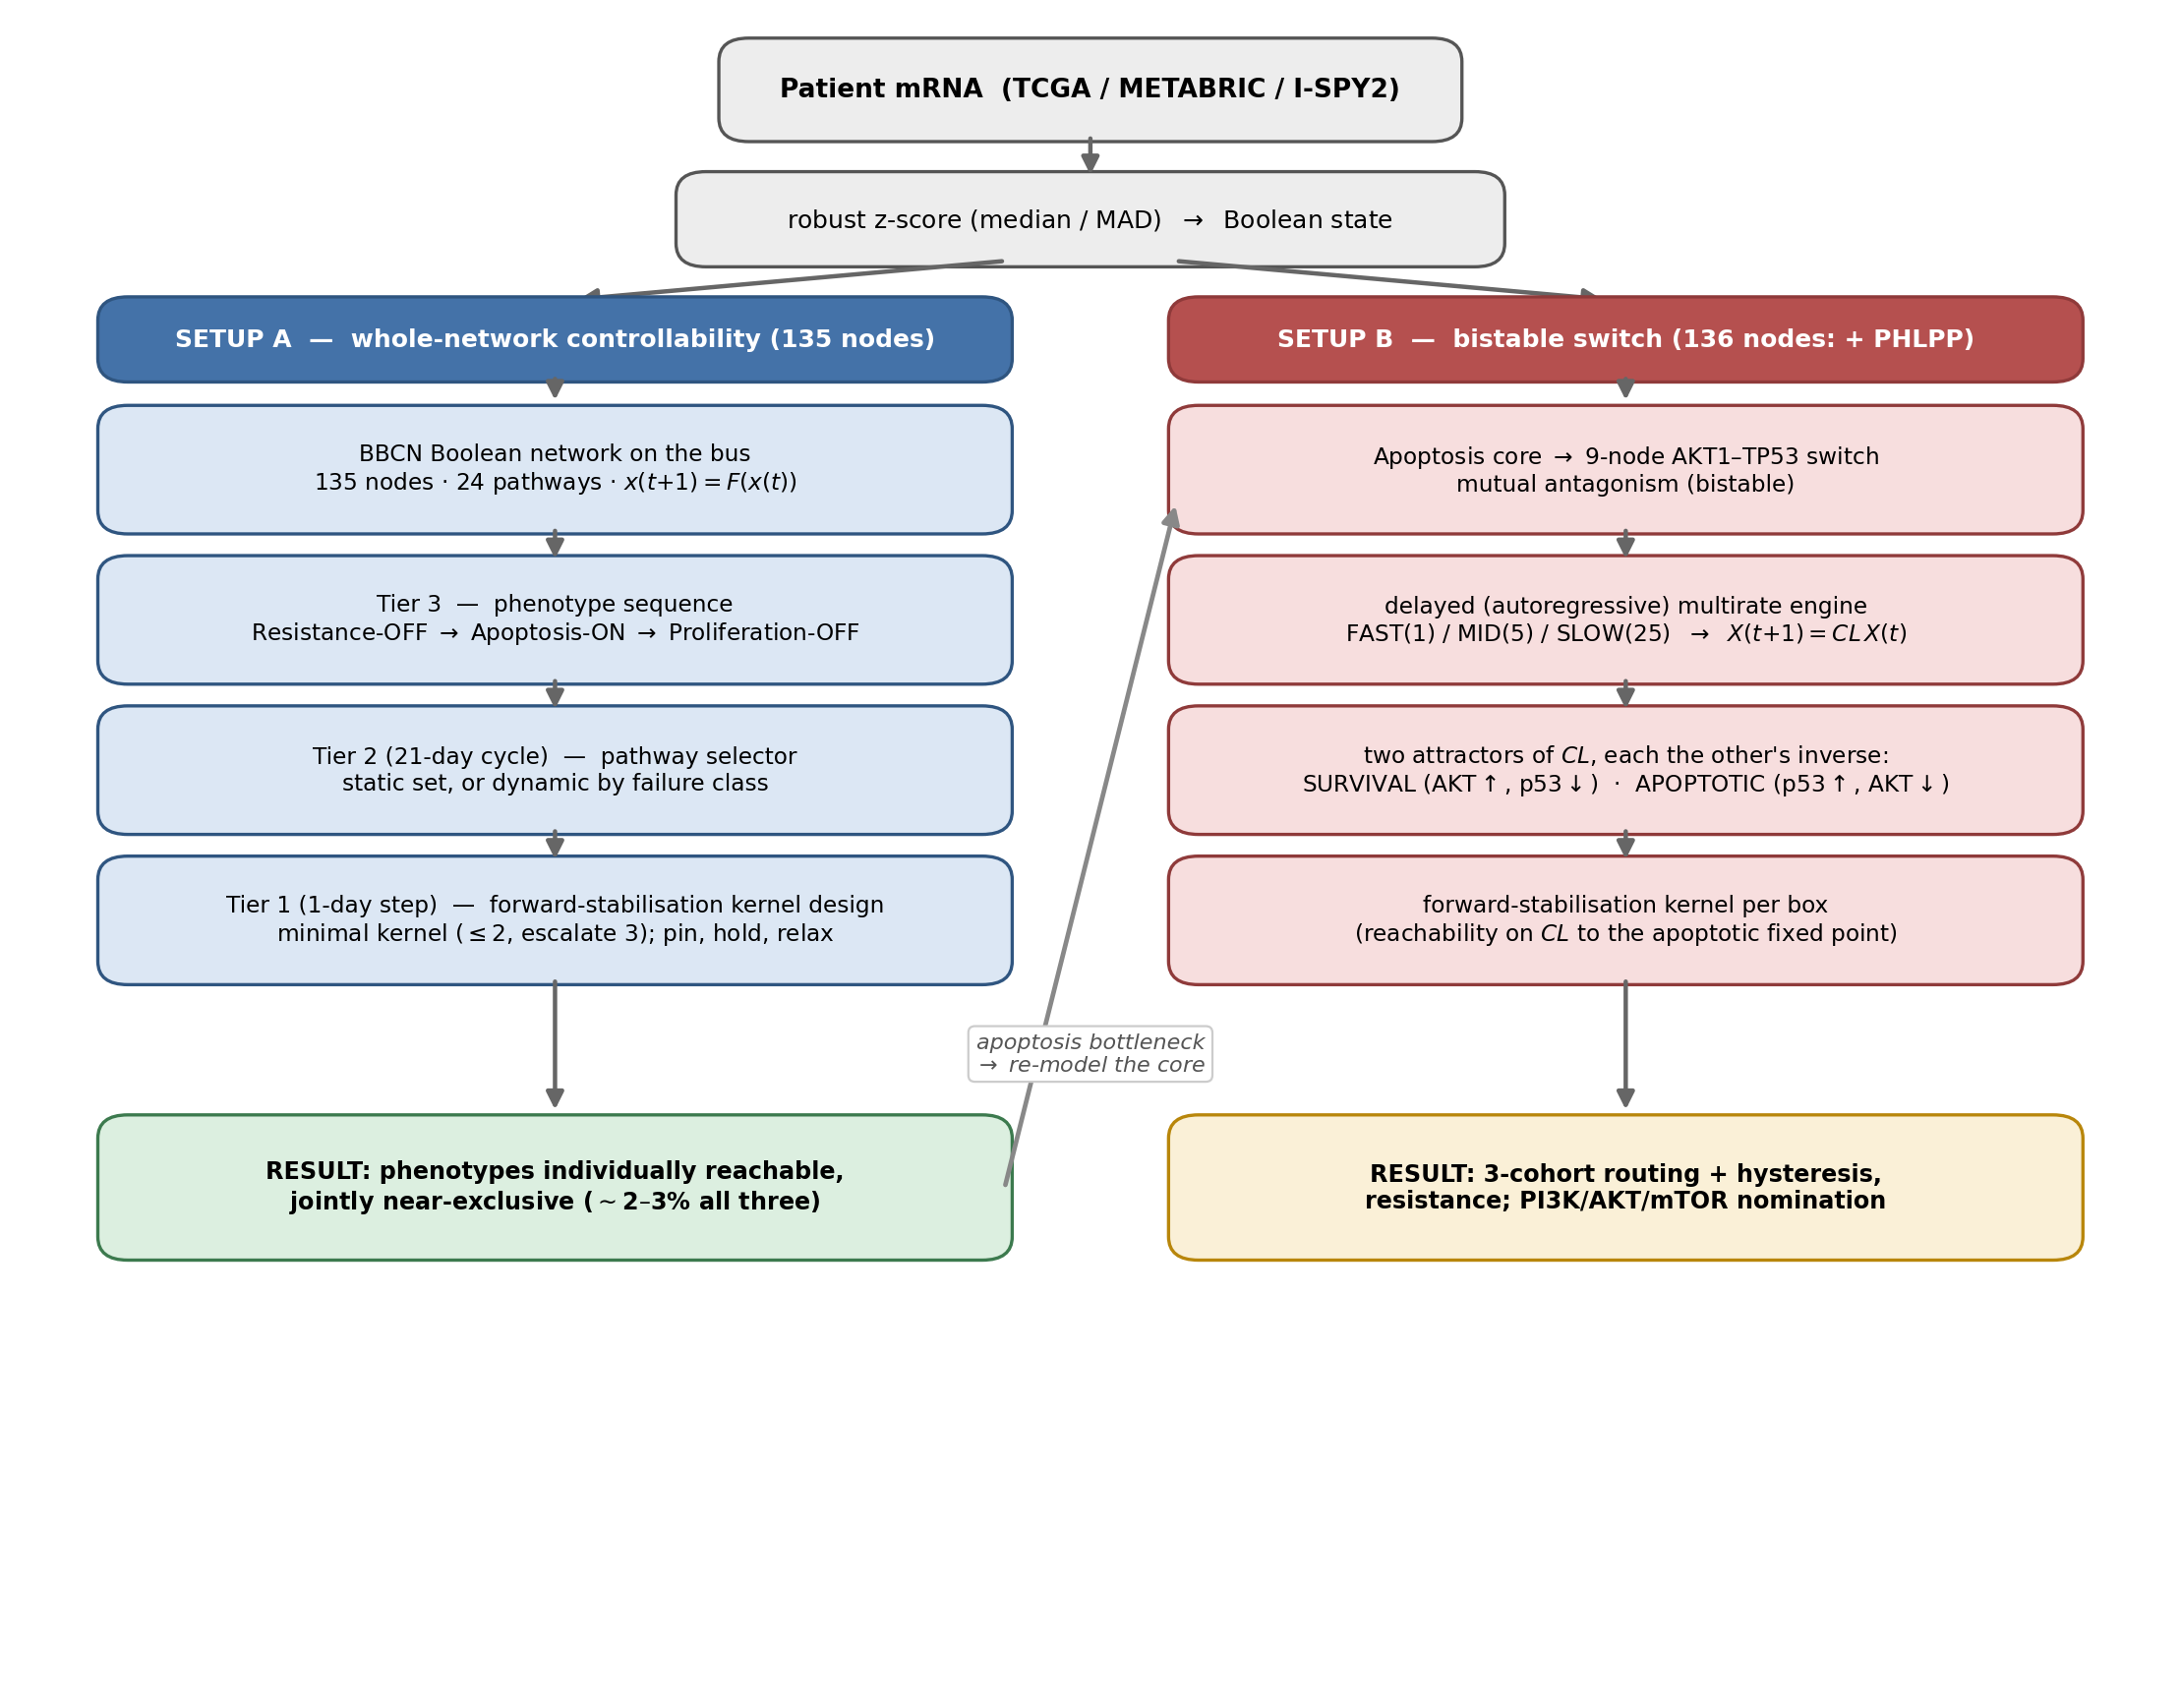
\includegraphics[width=\textwidth]{figures/fig_arch.png}
\caption{\textbf{The two setups of BBCN.} A shared front end binarises patient mRNA. Setup~A (left) drives the full 135-node network with a three-tier capped controller (phenotype sequencing $\rightarrow$ cycle-level pathway selection $\rightarrow$ day-level forward-stabilisation kernel design) and yields the controllability obstruction. Setup~B (right) re-models the apoptosis core as a 9-node AKT1--TP53 bistable switch, expressed as a delayed (autoregressive) multirate system (fast/mid/slow boxes on a 1:5:25 asynchronous schedule) with an STP algebraic form, then applies the same forward-stabilisation kernel design per box. The apoptosis bottleneck found in Setup~A motivates Setup~B.}
\label{fig:arch}
\end{figure}

% ------------------------------------------------------------
\section{Methods}

\subsection{Cohorts and patient-state initialisation}\label{sec:cohorts}
Patient states are derived from primary-tumour mRNA expression in three large public cohorts: TCGA-BRCA~\cite{tcga2012} (1082 patients, RNA-seq), METABRIC~\cite{metabric2012} (1980 patients, microarray), and I-SPY2 (988 patients, microarray; GEO GSE194040). The three cohorts were chosen to span different measurement platforms and different patient populations, so that any finding which holds across all three is unlikely to be an artefact of one assay or one centre. TCGA-BRCA and METABRIC are large primary-tumour reference cohorts on unrelated technologies, and I-SPY2 is a neoadjuvant trial cohort that also carries treatment annotation.

Each gene is converted to a Boolean value separately within each cohort. The activity score of a gene is its robust $z$-score, $(x-\mathrm{median})/(1.4826\cdot\mathrm{MAD})$, computed over all patients in that cohort, and the node is set ON when the score exceeds zero. The robust estimator is the default throughout. It uses the median and the median absolute deviation rather than the mean and the standard deviation, so a handful of extreme expression values, which are common in skewed RNA-sequencing data, cannot drag the threshold. Classic $z$-score and hard-median binarisation are retained only as alternatives for the sensitivity analysis, and the qualitative results do not depend on the choice.

Some nodes correspond to a signalling activity rather than to a single gene. For these, a curated multi-gene panel is reduced to one Boolean value by a majority vote: the node is ON when at least half of its panel genes are ON. The resulting Boolean vector, restricted to the network nodes, is the patient's initial state. The same front end feeds both setups, so Setup~A and Setup~B always see the identical binarised patient.

\subsection{The BBCN model and the two setups}
Two model instances are used and are kept clearly separated (Figure~\ref{fig:arch}). Setup~A is the 135-node network across 24 signalling pathway modules, used for the whole-network controllability analysis of Sections~\ref{sec:31} and \ref{sec:32}. Setup~B adds a single node, PHLPP, the phosphatase that closes the AKT--FOXO3a feedback the bistable switch requires, giving a 136-node model used for the switch analysis of Sections~\ref{sec:33} to \ref{sec:35}.

The two instances are one network seen at two resolutions, not two different models. PHLPP is dynamically inert outside the switch: with the switch logic disabled it neither drives nor is driven by the rest of the network, so the strongly-connected-component structure, the feasibility analysis, and the controllability results are bit-for-bit identical on the 135-node and the 136-node model. Setup~A is the whole network seen from the outside, and Setup~B is its apoptosis core seen from the inside.

The 135-node rule set is adapted substantially from the breast-cancer Boolean model of Taoma and colleagues~\cite{taoma2024}. Of the 135 nodes, 105 (78\%) correspond to nodes in that model, and once Taoma's merged complexes and isoforms are re-expressed here at individual-gene resolution (for example AKT1/2/3 as a single node there), the Boolean update rules coincide for the majority of the shared nodes. The present model extends that base from 117 to 135 nodes across 24 pathway modules, adding a DNA-damage arm (ATM, ATR, BRCA1/2, CHEK1/2), immune-checkpoint and NF-kB nodes, and the commitment-latch and PHLPP components the switch requires, and it builds on the author's earlier BBCN118 framework~\cite{bhatti2026}. The apoptosis and proliferation readouts, CASP3 and E2F1, follow Taoma's convention.

Each node is a gene or protein with a Boolean state and a logical update rule taken from the literature. The global state advances through a single synchronous map $x(t{+}1)=F(x(t))$. Pathways are modules of this one map and exchange signals only through the shared global state, which we call the bus; there is no hidden channel between pathways. Cell-fate phenotypes are read from the settled state as marker patterns: CASP3 for apoptosis, AKT1 for resistance, and CCND1 with E2F1 for proliferation. Throughout, an intervention may pin only its small kernel of nodes; everything else must move on its own, and a phenotype counts only when it is a genuine fixed point of the free dynamics.

\subsection{Setup A: the three-tier capped controller}
\paragraph{Three tiers on three timescales.} The controller is organised into three tiers, each acting on its own unit of time and its own unit of decision. Tier~3 sequences the target phenotypes in the clinical order resistance-OFF, then apoptosis-ON, then proliferation-OFF. Tier~2 acts on a 21-day clinical cycle, and its unit is pathways: from a candidate set it ranks pathways, upstream-first by default, and passes one or two of them down. Tier~1 acts on a single network step, taken as one day, and its unit is kernels: for each selected pathway it designs the minimal stabilising kernel and administers it. A cycle is one design step followed by relaxation. The kernel is fixed on day one and the network then evolves freely under it for the remainder of the cycle. The primary horizon is eight cycles, about six months; an extended horizon of seventeen cycles, about one year, is also available.

\paragraph{Caps and no accumulation.} The intervention is deliberately small. During induction up to two pathways act at once, giving four to five pinned nodes; during maintenance a single pathway gives two to three. The held kernel is re-decided at every cycle boundary and never exceeds the cap, and prior-cycle pins are not retained: the bus state carries forward but the intervention itself does not accumulate. This keeps the modelled therapy within a plausible drug-combination budget and prevents the controller from quietly clamping the whole network.

\paragraph{Two target families.} Targets are full-bus 135-node reference states, supplied in two families. The \emph{ideal} family encodes each phenotype as a standalone goal and is used for isolated, per-phenotype controllability. The \emph{compatible} family encodes protection-aware goals that, by construction, preserve phenotypes already achieved: the apoptosis target is compatible with resistance-OFF, and the proliferation target with both. Sequenced control uses the compatible family, so the all-three result measures whether the later phenotypes can be reached without giving back the earlier ones.

\paragraph{Kernel design.} The canonical kernel is the algebraic forward-stabilisation test of Rafimanzelat~\cite{rafimanzelat2025}. That test certifies \emph{global} stabilisation of a Boolean network to a target attractor; here it is applied at the finer granularity of the individual pathway module, with the per-module kernels composed sequentially. The conditions under which such local, pathway-wise stabilisation composes to a network-level result are the author's own weak-coupling pathway-decomposition theorem, introduced in the BBCN118 framework~\cite{bhatti2026} and restated in Appendix~\ref{app:theorem}. From a pathway's logical transition matrix $L$ and the state-modifying matrix $T_S^z$ that pins a candidate clamp set $S$ to its target values, one forms the controlled matrix $L_c=T_S^z L$, its transient power $\rho$, and the stabilisability matrix $\Omega=L_c^{\rho}\,T_S^z$. The set $S$ stabilises the pathway if and only if every column of $\Omega$ is the target's index vector, that is, clamping $S$ drives \emph{every} pathway state to target, not only the patient's current state. Candidate subsets are examined in increasing size, the smallest stabilising cardinality is taken, and among minimal stabilising sets ties are broken by least causal score and then lexicographically, which is a tiebreak only since every such set already stabilises. Because the test certifies global stabilisation, the algebraic kernel is independent of the pathway's own starting state, but it does depend on the pathway's external inputs: it is a function of the pathway rules, the current external-input snapshot, and the target. The kernel is therefore cached under the key (pathway, external snapshot, target) and rebuilt whenever the snapshot changes; reuse occurs only across patients, or cycles, that present the identical external snapshot. Because the inputs are binarised and each pathway reads only a few bus nodes, such snapshots recur across a cohort, so the cache still yields substantial reuse.

\paragraph{Exactness of the cached kernel.} The transition matrix $L$ is assembled from the pathway's rules with its external inputs held at their current values, so it is a snapshot of those inputs and is recomputed whenever they change as the network evolves; within a cycle the kernel is fixed, and it is refreshed at the next cycle boundary against the inputs as they then stand. The inputs that key this computation are the complete set of bus nodes the rules reference, read directly from the rules rather than discovered by probing a handful of states, so no live dependency is missed and the reuse is exact: two patients sharing an external snapshot share, provably, the same algebraic kernel. The ranked heuristic is handled differently, because it certifies reachability from the patient's own state and so its kernel depends on that state; it is recomputed afresh each cycle for each patient rather than reused.

\paragraph{A heuristic kept for continuity.} A ranked reachability heuristic, ordering candidates by impact, then improvement, then steps, then a causal score, is retained as a selectable alternative. It reproduces the kernels of the earlier BBCN118 framework exactly, and it is compared against the algebraic test (Section~\ref{sec:comparison}; full comparison in the Supplement), so the present controller stays continuous with the earlier method at the kernel level rather than replacing it silently.

\paragraph{What counts as success.} No node is ever forced. A phenotype is achieved only when its marker pattern holds at a genuine fixed point of the free dynamics under the held kernel. Progress within a run is tracked by a trajectory-based efficacy score, the time-averaged mismatch to target normalised by the initial mismatch, and each run is classified as recovered, stalled, or timed-out. Only recovered runs, those that reach a true fixed point, count toward the reported percentages.

\subsection{Setup B: the bistable switch as a delayed (autoregressive) multirate system}
\label{sec:methodsB}
Setup~A locates apoptosis inside a strongly coupled core that a whole-network controller cannot reliably reach (Section~\ref{sec:32}). Setup~B therefore models that core directly. The apoptosis core is a nine-node switch built on the mutual antagonism between AKT1, the survival hub, and TP53, the apoptosis hub. AKT1 represses p53 through MDM2, p53 represses AKT1 through PTEN, and a second arm runs $\lnot\mathrm{AKT1}\to\mathrm{FOXO3}\to\mathrm{PHLPP}\dashv\mathrm{AKT1}$. Two mutually repressing arms form a double-negative feedback loop, and a double-negative loop is the canonical source of bistability: the system settles into one of two self-consistent states, one with AKT1 high and p53 low, the other with p53 high and AKT1 low. The AKT1--FOXO3a arm resolves as follows. Active AKT phosphorylates FOXO3a, creating 14-3-3 docking sites that hold it in the cytoplasm and keep it transcriptionally silent, which the model captures as $\mathrm{FOXO3}=\lnot\mathrm{AKT1}$. When AKT activity falls, FOXO3a is dephosphorylated, enters the nucleus, and becomes transcriptionally active. The loop is closed in the model by making PHLPP FOXO3a-responsive: active FOXO3a sustains PHLPP, the phosphatase that dephosphorylates AKT~\cite{gao2005}, so low AKT begets active FOXO3a begets PHLPP begets lower AKT, a self-reinforcing negative loop that latches the state once entered. FOXO3a and p53 do not act as separate arms but as cooperating pro-apoptotic transcription factors: FOXO3a drives BIM ($\mathrm{BCL2L11}=\mathrm{FOXO3}\lor\mathrm{FOXO1}$) and both converge on APAF1 ($\mathrm{APAF1}=\mathrm{TP53}\lor\mathrm{FOXO1}\lor\mathrm{FOXO3}$), feeding the intrinsic caspase cascade. The two attractors are therefore internally consistent: the survival state carries AKT high with FOXO3a excluded and p53 held down by MDM2, and the apoptotic state carries AKT low with FOXO3a and p53 jointly active~\cite{wee2009}. The therapeutic question changes accordingly. Rather than push a marker against the coupled core, the task is to flip the switch from the survival state to the apoptotic state. \new{Commitment is latched by the intrinsic death cascade: p53 induces PUMA and NOXA, which repress BCL2/BCL-XL/MCL1; BAX and BAK permeabilise the mitochondrion; cytochrome c forms the apoptosome to activate CASP9; and CASP9 activates CASP3 once the IAP brake is removed. In the implemented model PUMA, NOXA and SMAC enter as derived intermediate terms rather than as formal updatable nodes, so the cascade nodes carried explicitly are BAX, BAK, CYCS, CASP9 and CASP3, and the node count is unchanged.}

\paragraph{Timescale as lag depth (the autoregressive form).}
Rather than impose a single clock, we encode biological timescale separation directly. The nine nodes are partitioned into three process classes: fast (AKT1, PTEN, MTOR, PDPK1, PIK3CA; phosphorylation), mid (MDM2; turnover), and slow (TP53, PHLPP, FOXO3; transcription). The slow regulators act at a delay, so the switch is a delay-difference recurrence over $\mathrm{GF}(2)$, an autoregressive Boolean model. Writing $a=\mathrm{AKT1}$, $m=\mathrm{MDM2}$, $p=\mathrm{TP53}$ and so on, the antagonism appears as a lagged negative loop, e.g.
\begin{equation}
\begin{aligned}
p(t{+}1) &= \lnot\, m(t-d_M)\ \lor\ \mathrm{ATM}(t)\ \lor\ \mathrm{ATR}(t),\\
a(t{+}1) &= \big(\mathrm{MTOR}\wedge \mathrm{PDPK1}\wedge \mathrm{PIK3CA}\big)(t)\wedge \lnot\mathrm{PTEN}(t)\wedge \lnot\mathrm{PHLPP}(t-d_S),
\end{aligned}
\end{equation}
where the lag depths $d_M,d_S$ are dimensionless integers, not rate constants. With non-zero lags the synchronous oscillation of the p53--MDM2 loop is broken: the slow feedback arrives delayed, so a sustained stress, rather than a transient, settles the cell into apoptosis. Equivalently, the model is run as an asynchronous multirate schedule in the ratio $1{:}5{:}25$, in which the fast box updates every step, the mid box every five steps, and the slow box every twenty-five, with all firing boxes reading a common pre-update snapshot. The lag form and the multirate schedule are two views of the same timescale separation; neither uses continuous values, Hill functions, or time constants.

\paragraph{Why the durable death state is structural, not a scheduling artifact.}
A reasonable objection is that Setup~A's inability to hold apoptosis is merely an artifact of synchronous updating, and that the multirate schedule of Setup~B simply removes that artifact. It is not, and the reason is that a fixed point is invariant to the update scheme: a state with $f(x)=x$ is a fixed point under synchronous, asynchronous, or multirate updating alike. Whether a durable apoptotic state exists is therefore a structural question, not a question of the clock. Two checks settle it. First, the free 135-node dynamics of Setup~A carry essentially no fixed-point attractors in the reachable region: started from patient resting states they fall into limit cycles rather than fixed points, and node-level random-order asynchronous updating does not settle them either, so the oscillation is a property of the network and not of synchronous timing. There is consequently no apoptotic fixed point for any schedule to reach. Second, the apoptotic state of the Setup~B switch is a genuine synchronous fixed point of its rules, present for the subset of patients whose input configuration admits it, and the designed kernel drives the patient exactly onto that fixed point. The multirate schedule therefore governs convergence, letting a trajectory settle onto the latch rather than oscillate on the way in, while the durability of the destination is a structural property of the bistable core that holds under any update scheme. This is also why durability and feasibility coincide in Setup~B but not in Setup~A: the patients for whom the death state exists are exactly those for whom a withdrawable pulse leaves the cell apoptotic.
\authornote{the resting-state attractor census for Setup~A and the synchronous fixed-point enumeration for the Setup~B switch are to be added to the reproducible pipeline and their counts macro-sourced alongside the other numbers.}

\paragraph{STP algebraic form and control.}
Using the semi-tensor product, each rule has a structure matrix and the delayed system admits a linear algebraic form. The delay is removed by state augmentation: lifting $X(t)=x(t)\ltimes x(t{-}1)\ltimes\cdots\ltimes x(t{-}d)$ gives the delay-free companion form
\begin{equation}
X(t{+}1)=C_L\cdot X(t),
\end{equation}
the standard delay-to-companion-form lift. The fixed points are the unit-diagonal columns of the input-absorbed transition operator; for this switch there are exactly two, the survival state (AKT1, MDM2 high; the rest low) and the apoptotic state (its complement), recovering by linear algebra the two attractors found by direct enumeration. Steering a patient from the survival to the apoptotic fixed point is then a reachability problem on this operator. Because the lifted dimension grows with the delay, the lags are kept small. The same forward-stabilisation kernel method as Setup~A is applied per timescale box, with the druggable actuators restricted to the fast survival nodes and the genotoxic/stress inputs (ATM, ATR, E2F1) treated as a separate actuator class.

\subsection{The three biological repairs and the biology-faithful network}
\label{sec:repairs}
The baseline network of Setup~A is globally oscillatory and supports no durable apoptotic fixed point. We trace this to three pieces of degenerate feedback wiring and restore each to its textbook form. These three simplifications are of a kind common in literature Boolean models of this scope, where such abstractions are appropriate to the drug-response questions those models address; we do not treat them as errors. They become limiting only for the durability question posed here, and restoring them, with no parameter tuning, is what converts a non-durable, oscillatory network into one that supports durable, controllable apoptosis. The repairs are applied as an overlay: the baseline \texttt{pathways.py} is untouched, so the original network is preserved and either network can be selected by a single call. The biology-faithful network is the baseline 135-node network plus PHLPP, giving 136 signalling nodes; the staged-controller branch additionally carries a commitment-latch node and a per-patient uncoupling flag.

\emph{R1. p53--MDM2--ATM damage sensor.} In the baseline rules MDM2 is held high by a self-loop and TP53 reads only the negation of MDM2, with no damage input, so p53 activity is identically zero whatever the damage. The repair restores the canonical sensor, $\mathrm{MDM2}=(\mathrm{TP53}\lor\mathrm{AKT1})\land\lnot(\mathrm{CDKN2A}\land(\mathrm{E2F1}\lor\mathrm{ATM}\lor\mathrm{ATR}))$ and $\mathrm{TP53}=\lnot\mathrm{MDM2}\lor\mathrm{ATM}\lor\mathrm{ATR}$, so damage through ATM or ATR stabilises p53.

\emph{R2. AKT1--FOXO3a--PHLPP loop and the uncoupling flag.} The baseline AKT--FOXO arm has no closing feedback. The repair adds PHLPP, the phosphatase that closes the loop, and a flag $U$ that marks cells in which AKT activity and nuclear FOXO co-occur, the resistant configuration, the AKT--FOXO3a uncoupling documented as a breast-cancer resistance signature~\cite{brunet1999,chen2010}; $U$ is computed per patient from the binarised state, not assumed.

\emph{R3. Death-engaged commitment latch.} Apoptotic commitment is irreversible past a point. We add an integrator that accumulates only when death is winning, when p53 is high and AKT is down together, and that on crossing a threshold latches a commitment which releases the survival brakes (MCL1, XIAP, CFLAR, BCL2, BCL2L1). Integrating raw p53 instead destroys the switch's bistability, because the uncoupled resistant state carries high p53 yet survives; the death-engaged form preserves it.

\subsection{Validation and reproducibility}
Two kinds of check are applied. First, the nominated kernel genes are compared against curated clinical drug-target evidence (CIViC) and against cohort mutation data, and the switch routing is tested for outcome alignment on the treatment-annotated I-SPY2 trial. Second, the drug-target nomination is repeated through three independent front-ends, median-binarised expression, multi-gene activity signatures, and phospho-protein activity, to confirm that it does not depend on one way of reading the data. The scope is stated honestly. No survival benefit is claimed; the recommended axis was largely not administered to these chemo-era patients, so there is no response-validation cohort; the analysis is on primary tumours only; and invasion is left out of scope because the network carries too few of the canonical drivers to support it.

Both setups regenerate their headline numbers deterministically with a single command. To respect the terms of the source datasets, only the TCGA-BRCA binarised inputs are redistributed with the code; METABRIC is under controlled access (European Genome-phenome Archive; processed data via cBioPortal under its data-use terms) and the I-SPY2 inputs are obtainable from GEO series GSE194040. For those two cohorts the repository documents the binarisation procedure (the robust z-score of Section~\ref{sec:cohorts}) rather than shipping the patient-level matrices, so a user with the primary data regenerates the inputs and reproduces every number; TCGA-BRCA alone runs the pipeline out of the box. Setup~A self-verifies against a committed reference table, and the switch pipeline is deterministic, so the same inputs always produce the same numbers. Every number, figure, and table in this report was produced by these runs, and the manuscript reads its numbers from the generated file rather than transcribing them by hand, so the text and the code cannot drift.
\authornote{the formal STP / delayed-BCN treatment (structure matrices, controllability matrix) and the full nine-node rule table will go to a Supplementary Information section; the decomposition theorem of the prior work is cited, not reproduced.}

% ------------------------------------------------------------
\section{Results}

\subsection{Phenotypes are individually controllable but jointly near-exclusive}
\label{sec:31}
Under the three-tier capped controller, each phenotype is highly controllable on its own. Driving apoptosis-ON from the patient's state reaches a genuine fixed point in \BBCNAStaticRankedTcgaIsoApoptosisOn\% of TCGA, \BBCNAStaticRankedMetabricIsoApoptosisOn\% of METABRIC, and \BBCNAStaticRankedIspyTwoIsoApoptosisOn\% of I-SPY2 patients, and proliferation-OFF in \BBCNAStaticRankedTcgaIsoProliferationOff\%, \BBCNAStaticRankedMetabricIsoProliferationOff\%, and \BBCNAStaticRankedIspyTwoIsoProliferationOff\% respectively. These rates sit close together across three platforms and two patient populations, so individual controllability is a property of the network rather than of one cohort. Resistance-OFF is the hardest single phenotype everywhere (\BBCNAStaticRankedTcgaIsoResistanceOff\%, \BBCNAStaticRankedMetabricIsoResistanceOff\%, \BBCNAStaticRankedIspyTwoIsoResistanceOff\%), a first sign that the survival axis is held in place by the rest of the network.

The picture inverts when the three phenotypes are pursued in sequence with the compatible targets, which require that each new phenotype be reached without surrendering the ones already won. Success collapses to \BBCNAStaticRankedTcgaSeqAllThree\% in TCGA, \BBCNAStaticRankedMetabricSeqAllThree\% in METABRIC, and \BBCNAStaticRankedIspyTwoSeqAllThree\% in I-SPY2 (Table~\ref{tab:setupA}). The distance between the high isolated numbers and the low joint number is the central observation of Setup~A: the phenotypes are each feasible, yet they cannot be held at the same time. Because success is defined as a genuine free-dynamics fixed point with no node forced, this is not an artefact of pinning too few nodes; it is a statement about where the network is able to rest. The next section shows why.

\begin{table}[h]
\centering
\caption{Setup~A controllability (\% of patients reaching a genuine fixed point).}
\label{tab:setupA}
\begin{tabular}{lcccc}
\toprule
Cohort / regime & Resistance & Apoptosis & Proliferation & All three \\
\midrule
TCGA, isolated   & \BBCNAStaticRankedTcgaIsoResistanceOff & \BBCNAStaticRankedTcgaIsoApoptosisOn & \BBCNAStaticRankedTcgaIsoProliferationOff & n/a \\
TCGA, sequenced  & \BBCNAStaticRankedTcgaSeqResistanceOff & \BBCNAStaticRankedTcgaSeqApoptosisOn  & \BBCNAStaticRankedTcgaSeqProliferationOff  & \BBCNAStaticRankedTcgaSeqAllThree \\
METABRIC, isolated  & \BBCNAStaticRankedMetabricIsoResistanceOff & \BBCNAStaticRankedMetabricIsoApoptosisOn & \BBCNAStaticRankedMetabricIsoProliferationOff & n/a \\
METABRIC, sequenced & \BBCNAStaticRankedMetabricSeqResistanceOff & \BBCNAStaticRankedMetabricSeqApoptosisOn  & \BBCNAStaticRankedMetabricSeqProliferationOff  & \BBCNAStaticRankedMetabricSeqAllThree \\
I-SPY2, isolated  & \BBCNAStaticRankedIspyTwoIsoResistanceOff & \BBCNAStaticRankedIspyTwoIsoApoptosisOn & \BBCNAStaticRankedIspyTwoIsoProliferationOff & n/a \\
I-SPY2, sequenced & \BBCNAStaticRankedIspyTwoSeqResistanceOff & \BBCNAStaticRankedIspyTwoSeqApoptosisOn  & \BBCNAStaticRankedIspyTwoSeqProliferationOff  & \BBCNAStaticRankedIspyTwoSeqAllThree \\
\bottomrule
\end{tabular}
\end{table}

This pattern is not an average over receptor subtypes. We repeated the analysis on the receptor-low subset, defined by ESR1, PGR, and ERBB2 all low in the binarised data as a transcriptomic proxy for triple-negative status, which is the subtype closest to the basal-like patients of the earlier framework. The subset is 18 to 28\% of each cohort. Individual controllability is preserved or slightly higher there (apoptosis 75 to 91\%, proliferation 95 to 98\%), while the joint all-three rate stays in the low single digits (1 to 3\%), exactly as in the full cohort (Figure~\ref{fig:tnbc}). The feasibility-versus-reachability gap is therefore a property of the network, not of one receptor subtype.

\begin{figure}[h]
\centering
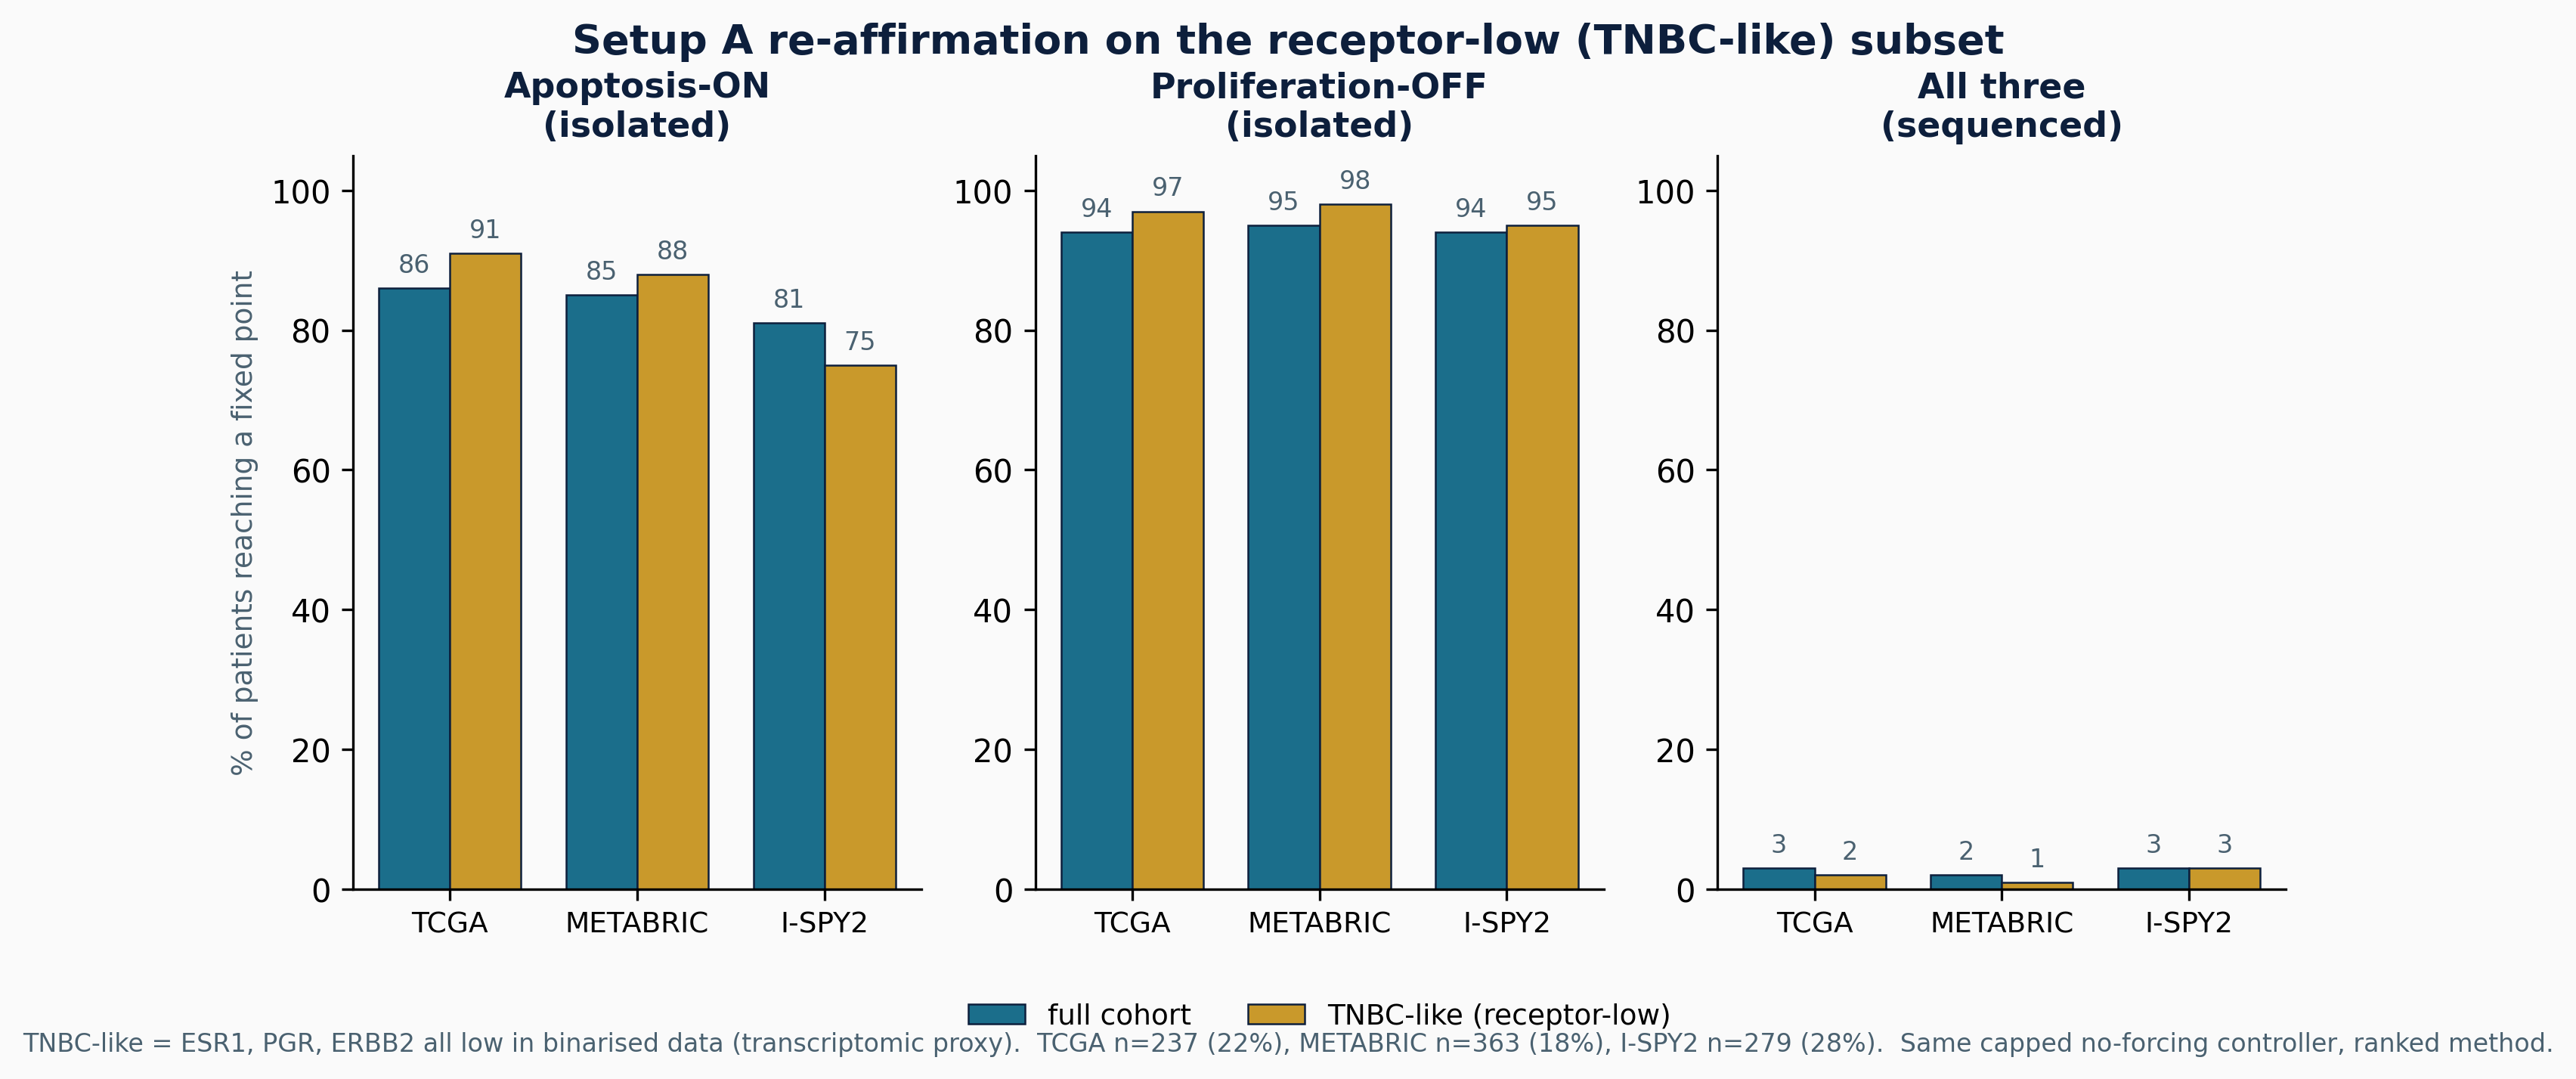
\includegraphics[width=\textwidth]{figures/figA_tnbc_panel.png}
\caption{\textbf{Re-affirmation on the receptor-low (TNBC-like) subset.} The Setup A static controller (ranked) on the full cohort (teal) and on the receptor-low subset (gold), the latter defined by low ESR1, PGR, and ERBB2 in the binarised data as a transcriptomic proxy for triple-negative status. Individual phenotypes remain highly controllable in the subset while the joint all-three rate stays in the low single digits, the same individual-versus-joint pattern as in the full cohort. Subset sizes: TCGA 237 (22\%), METABRIC 363 (18\%), I-SPY2 279 (28\%).}
\label{fig:tnbc}
\end{figure}

\subsection{The obstruction is a dominant strongly-connected core}
\label{sec:32}
The reason is structural. We build a directed coupling graph whose nodes are the 22 regulatory pathways, with an edge from one pathway to another when a node in the first appears in the update rule of the second, and we compute its strongly-connected components with Tarjan's linear-time algorithm~\cite{tarjan1972}. A strongly-connected component is a set of pathways that all feed back into one another, so a signal injected anywhere in it can circulate to every member. The graph is dominated by one such component of 16 pathways, with a secondary component of two; together about 82\% of the regulatory pathways lie inside cyclic cores rather than in a clean feed-forward chain (Figure~\ref{fig:scc}).

The coupling is distributed, not funnelled through a single hub. The strongest carriers are AKT1, MAPK1, FOXO3, and TP53, but removing the AKT1 coupling shrinks the dominant component only from 16 pathways to 14, so no one or two ablations break the cycle. This is exactly the regime in which pathway-by-pathway stabilisation fails. Stabilising a pathway in isolation is sound only on a weakly coupled, acyclic network; inside a strongly-connected core the other members re-inject the very signals an intervention removes, so a phenotype can be feasible yet unreachable under any bounded, non-accumulating budget. This also locates the boundary of the earlier BBCN118 decomposition theorem, which holds under weak inter-pathway coupling: the full network does not meet that condition on the hard case, which is why the sequenced result collapses, and why the apoptosis core must be modelled on its own terms in Setup~B.

\begin{figure}[h]
\centering
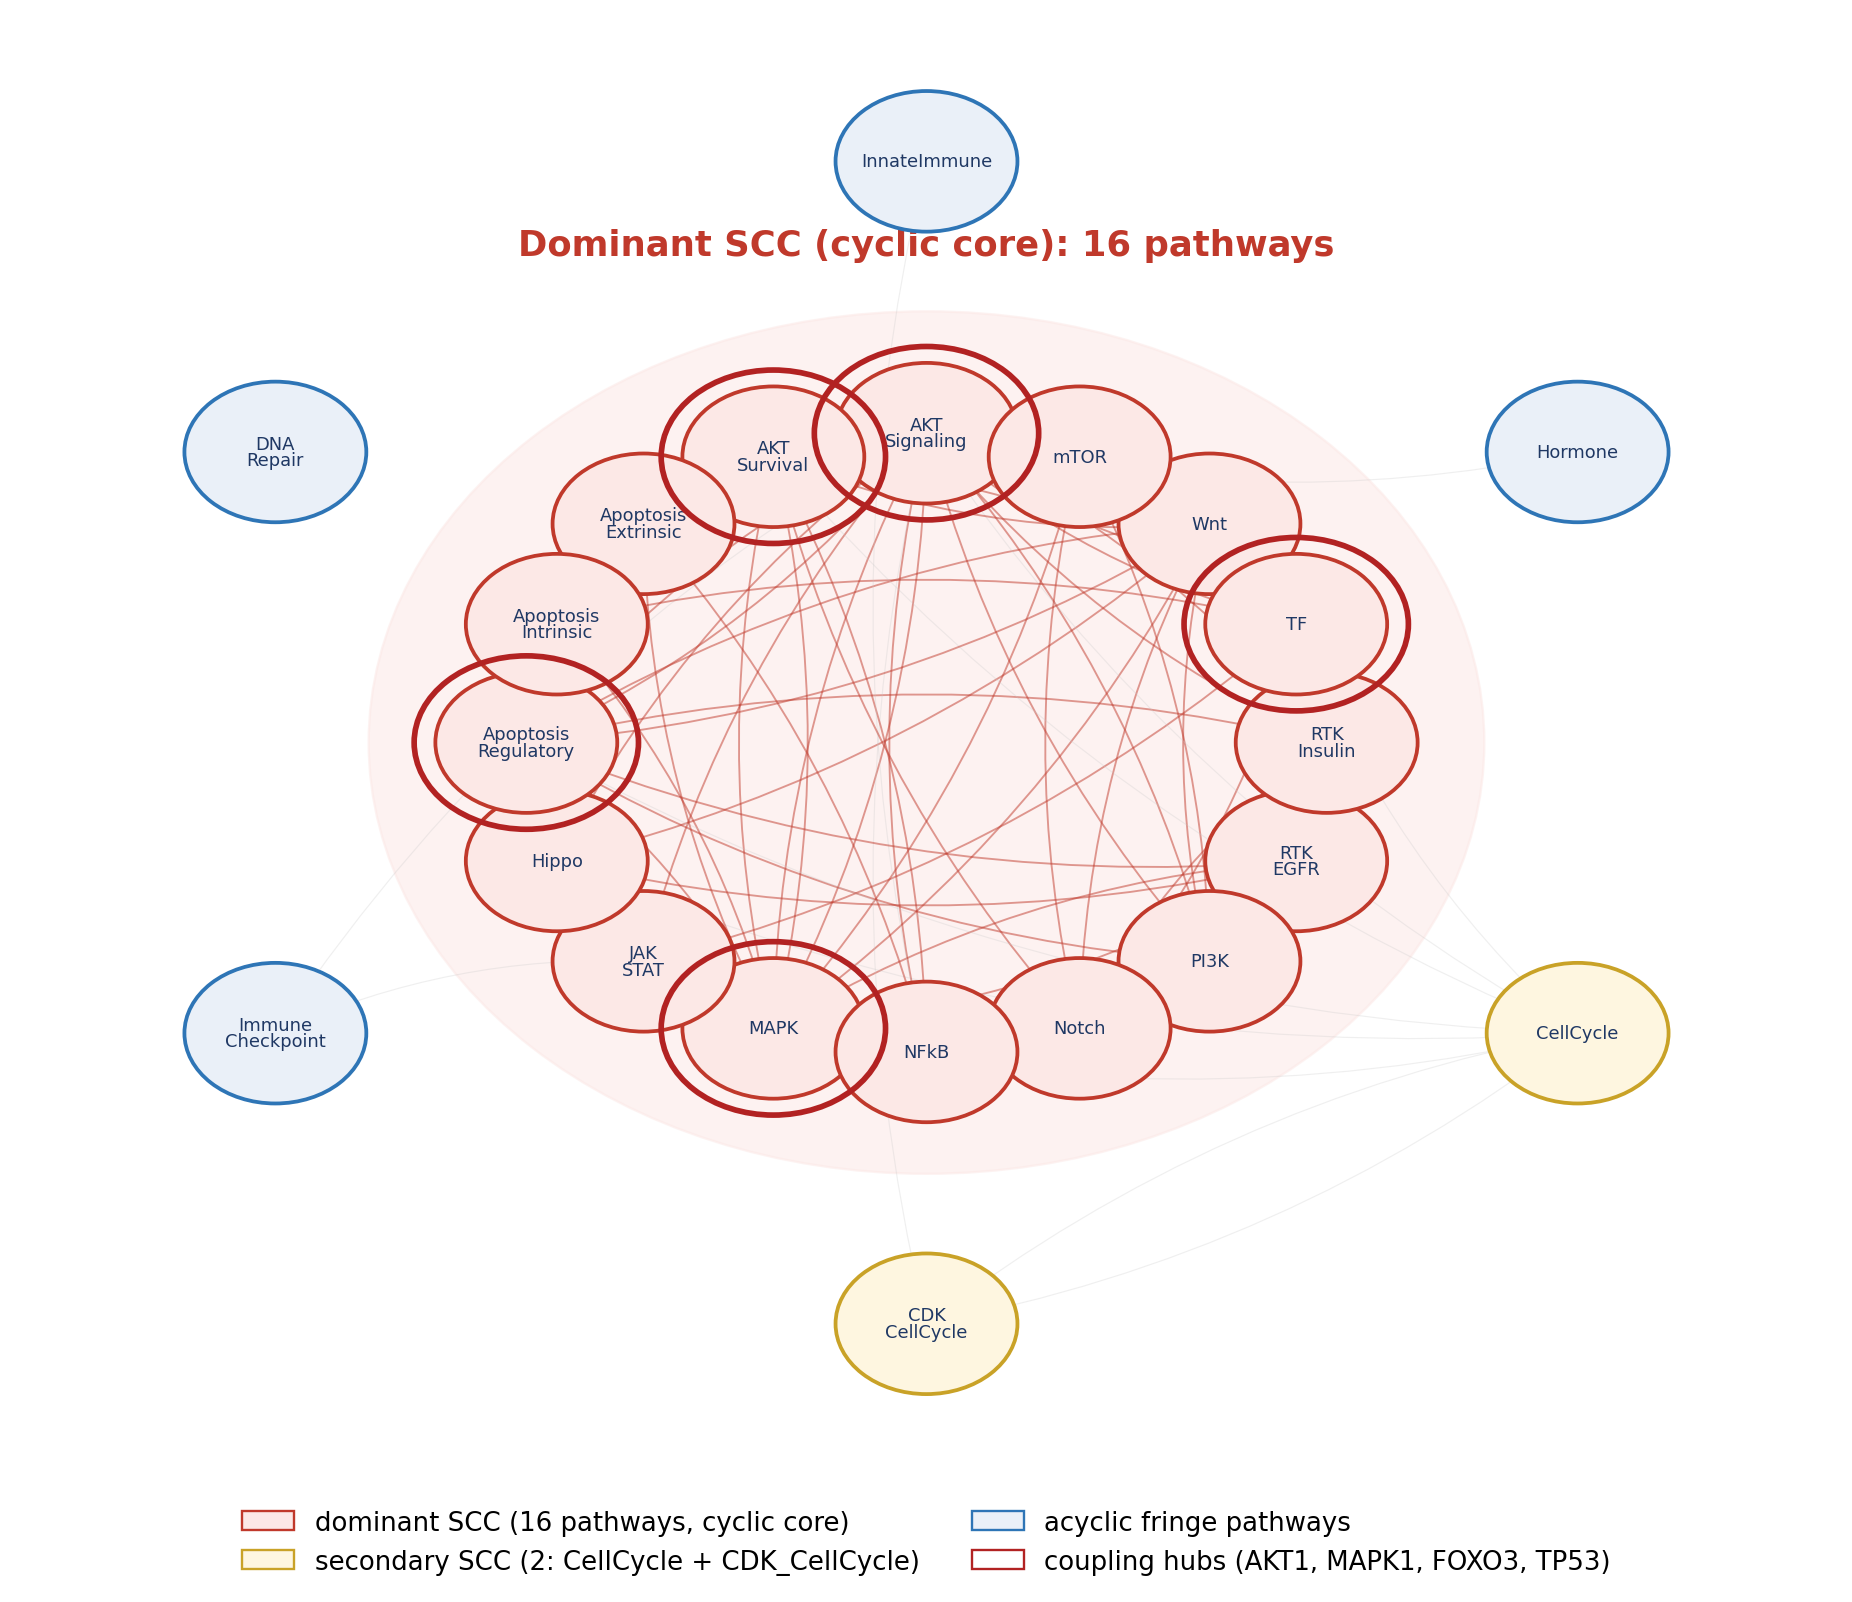
\includegraphics[width=0.6\textwidth]{figures/fig2_scc.png}
\caption{\textbf{The pathway coupling graph.} The dominant 16-pathway strongly-connected component is shaded as the cyclic core; the coupling hubs (AKT1, MAPK1, FOXO3, TP53) are ringed. The two auxiliary input modules are excluded.}
\label{fig:scc}
\end{figure}

Where control is \emph{applied} is itself modular, which sharpens the obstruction rather than softening it. Mapping each designed kernel to the pathway it serves gives a near block-diagonal pattern (Figure~\ref{fig:kernelAblock}): each actuator acts within its own pathway module, with little off-diagonal leakage, so the interventions are sparse and pathway-confined. Yet the free dynamics still carry their effects around the cyclic core, so this local, pathway-wise application does not translate into joint reachability. Sparse modular control inside a strongly-coupled core is exactly the regime in which pathway-by-pathway stabilisation is sound locally but fails globally.

\begin{figure}[htbp]
\centering
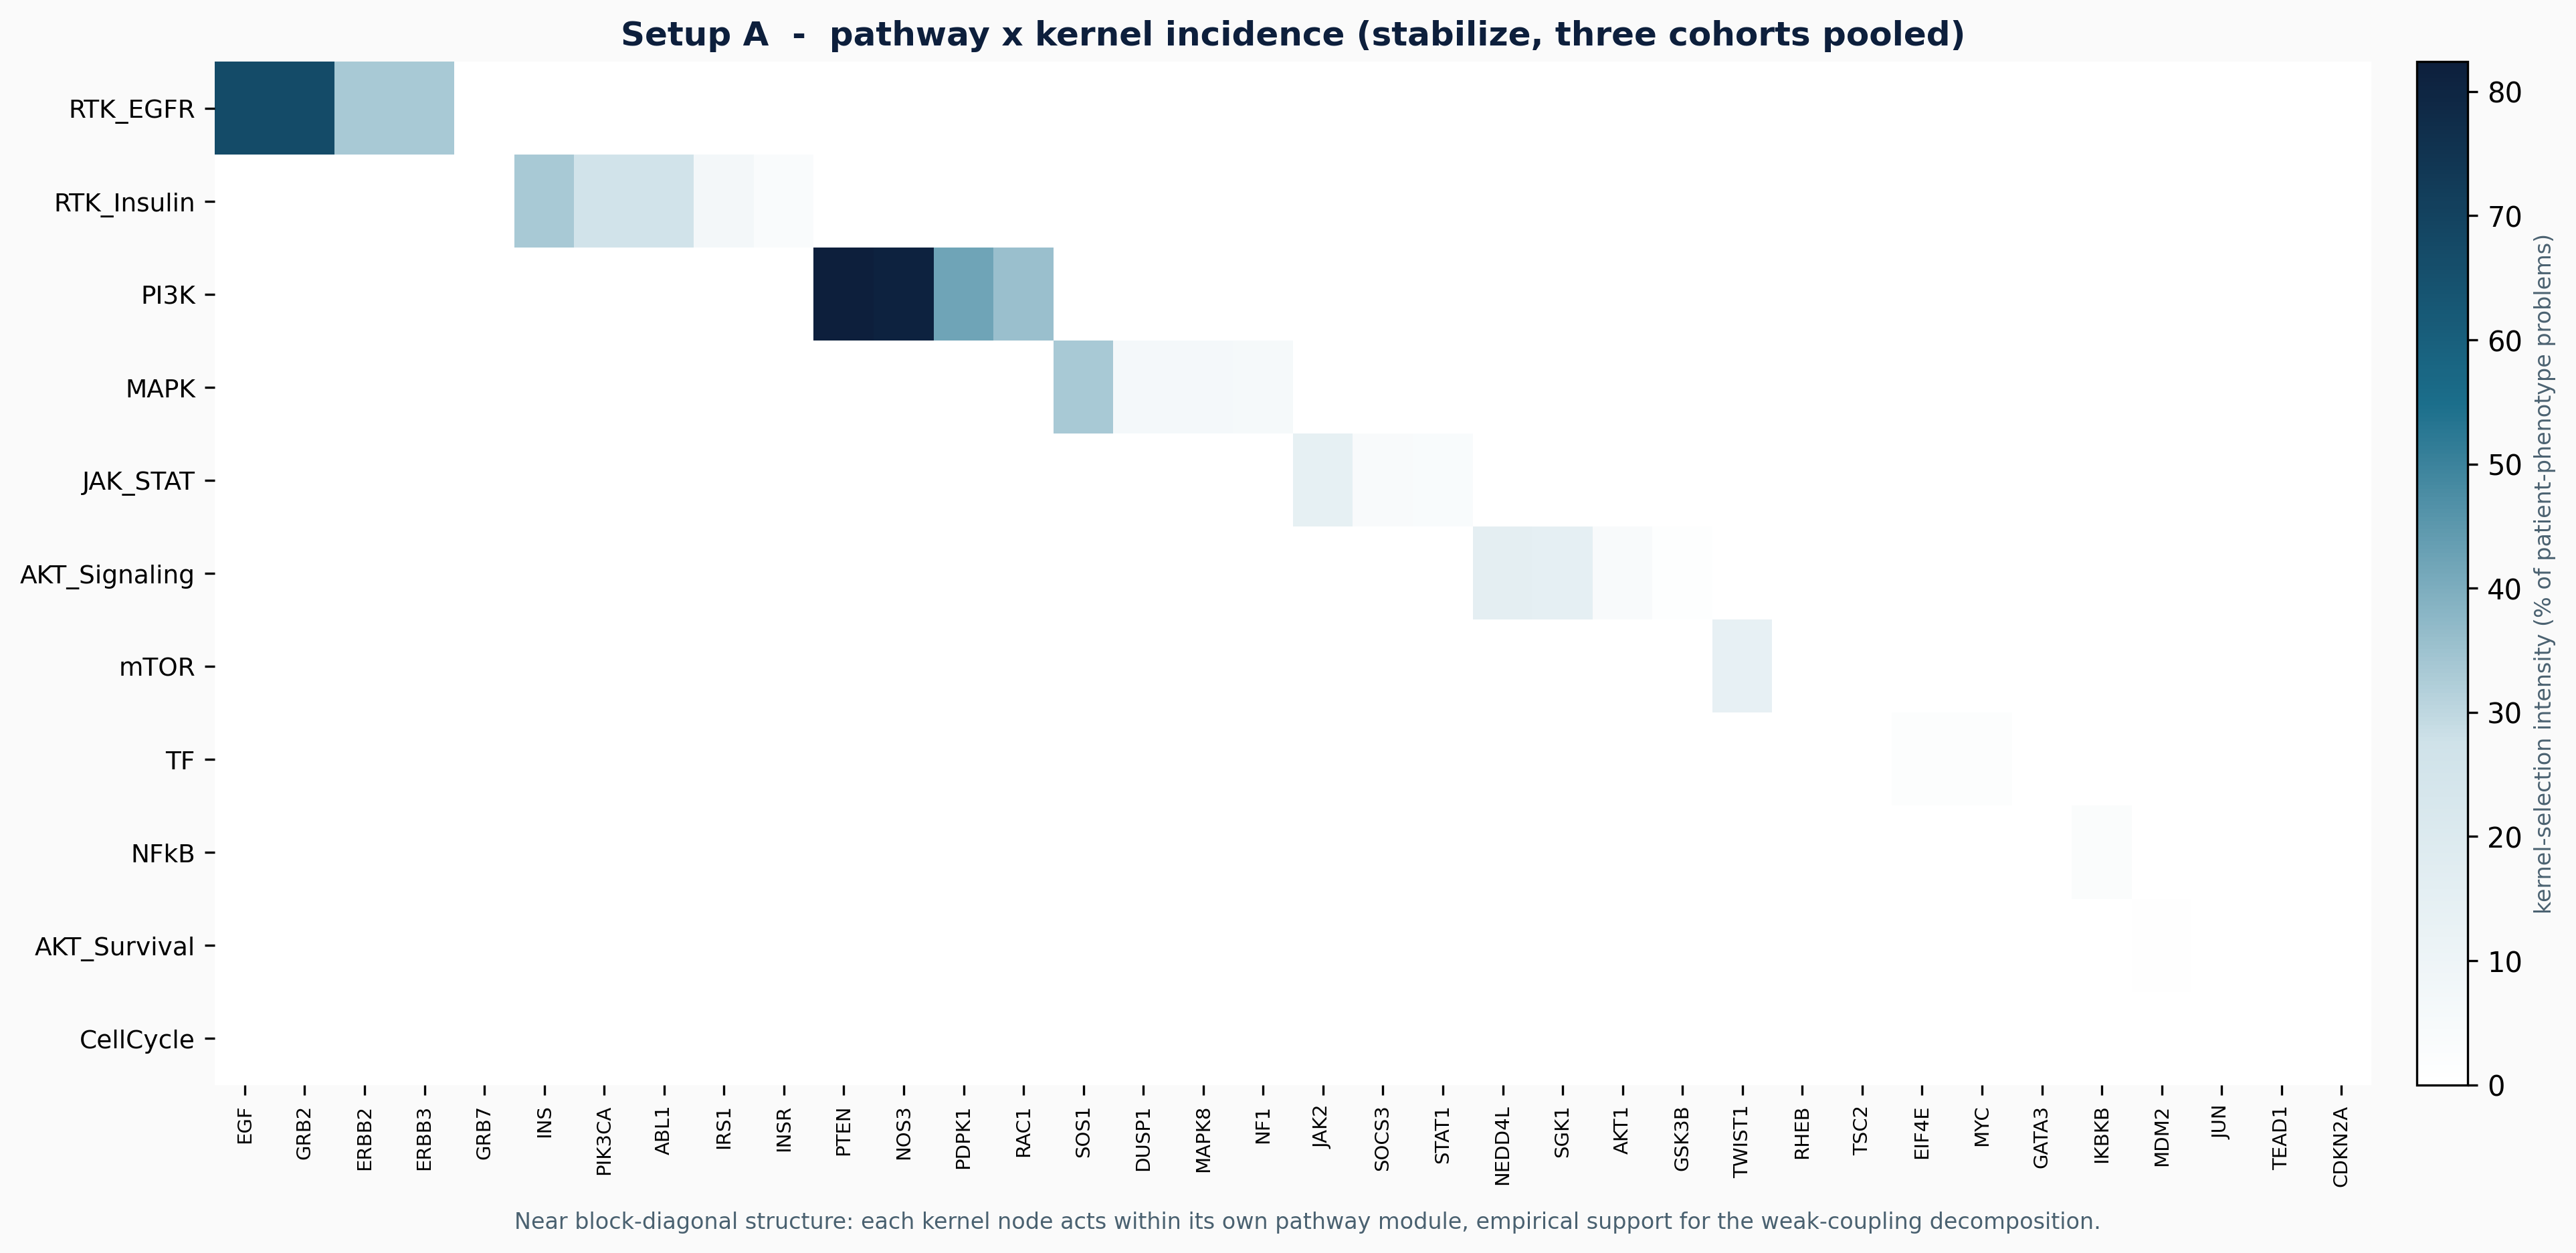
\includegraphics[width=\textwidth]{figures/figA_pathway_kernel.png}
\caption{\textbf{Setup~A pathway-by-kernel incidence: control is modular.} Kernel-selection intensity for each pathway and node pair, pooled over the three cohorts under the algebraic test. The near block-diagonal structure shows that each kernel node acts inside its own pathway module: RTK kernels on EGF, GRB2, and ERBB2; the PI3K kernel on PTEN, NOS3, and PDPK1; MAPK on SOS1, DUSP1, and NF1; JAK--STAT on JAK2 and SOCS3; AKT on NEDD4L, SGK1, and AKT1; and mTOR on TWIST1 and RHEB. Interventions are sparse and pathway-confined; their effects nonetheless propagate through the coupled core of Figure~\ref{fig:scc}, which is why modular application does not yield joint reachability.}
\label{fig:kernelAblock}
\end{figure}

\subsection{A bistable switch resolves the apoptosis core and routes patients coherently}
\label{sec:33}
Re-modelled as a bistable switch, the apoptosis core has two stable attractors: a survival state with AKT high and p53 low, and an apoptotic state with p53 high and AKT low. The control problem becomes flipping the switch rather than pushing a marker against the coupled core. Each patient's binarised state seeds the switch, which is run on the multirate schedule until it settles. Across the three cohorts the switch routes about half of patients to the apoptotic attractor (\BBCNBRoutingSwitchTcgaApopPct\%, \BBCNBRoutingSwitchMetabricApopPct\%, \BBCNBRoutingSwitchIspyTwoApopPct\% for TCGA, METABRIC, and I-SPY2), about a quarter to the survival attractor (\BBCNBRoutingSwitchTcgaSurvPct\%, \BBCNBRoutingSwitchMetabricSurvPct\%, \BBCNBRoutingSwitchIspyTwoSurvPct\%), and the remainder to a mixed outcome (Figure~\ref{fig:switch}, Table~\ref{tab:setupB}). The split is stable across the three platforms, so it is not a feature of one assay.

The routing is biologically coherent, which is what makes it more than a relabelling. Survival-routed patients are \BBCNBRoutingSwitchTcgaSurvUncoupledPct\%, \BBCNBRoutingSwitchMetabricSurvUncoupledPct\%, and \BBCNBRoutingSwitchIspyTwoSurvUncoupledPct\% in the uncoupled AKT--FOXO3a resistant state, against cohort-wide rates of \BBCNBRoutingSwitchTcgaUPct\%, \BBCNBRoutingSwitchMetabricUPct\%, and \BBCNBRoutingSwitchIspyTwoUPct\%, an enrichment of roughly threefold, and a multidrug-resistance signature is higher in the survival-routed group than in the apoptotic-routed group in every cohort. In other words, the switch sends precisely the biologically resistant patients to the survival attractor. That is a falsifiable prognostic alignment rather than an arbitrary partition: it states in advance which patients the model expects to resist apoptosis, and that prediction can be checked against independent resistance markers.

\begin{figure}[h]
\centering
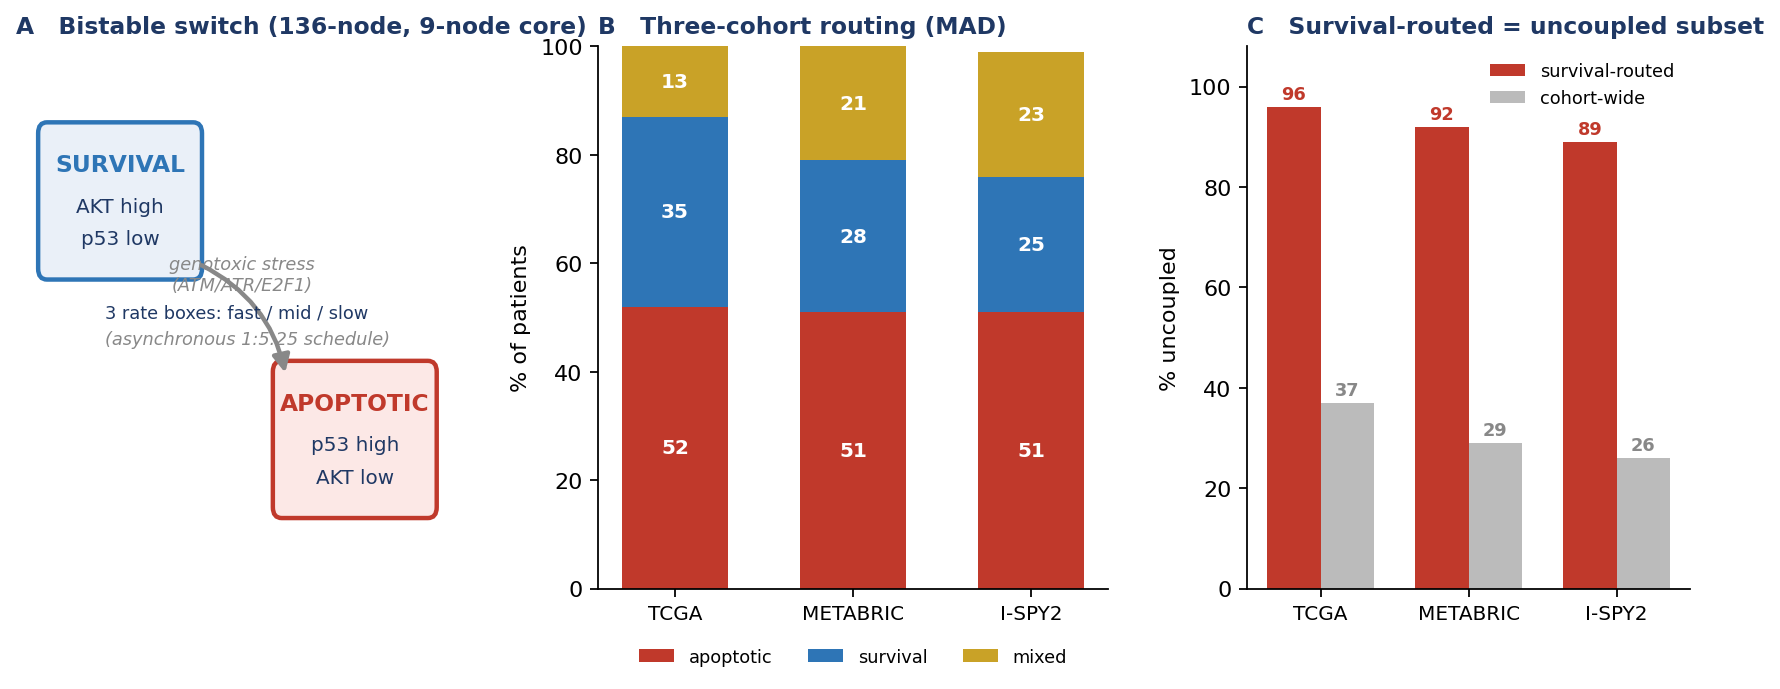
\includegraphics[width=\textwidth]{figures/figB.png}
\caption{\textbf{The bistable switch (136-node model).} (A) The two attractors and the survival$\to$apoptosis flip under sustained genotoxic stress. (B) Three-cohort routing (robust $z$-score): about half apoptotic, a quarter survival, the rest mixed, consistent across platforms. (C) Biological check: survival-routed patients are 89--95\% uncoupled, versus 26--37\% cohort-wide.}
\label{fig:switch}
\end{figure}

\begin{table}[h]
\centering
\caption{Setup~B switch routing and biological check (robust $z$-score, full cohorts).}
\label{tab:setupB}
\begin{tabular}{lcccc}
\toprule
Cohort ($N$) & Apoptotic & Survival & Mixed & SURV uncoupled \\
\midrule
TCGA (\BBCNBRoutingSwitchTcgaN)    & \BBCNBRoutingSwitchTcgaApopPct\% & \BBCNBRoutingSwitchTcgaSurvPct\% & \BBCNBRoutingSwitchTcgaMixedPct\% & \BBCNBRoutingSwitchTcgaSurvUncoupledPct\% vs \BBCNBRoutingSwitchTcgaUPct\% \\
METABRIC (\BBCNBRoutingSwitchMetabricN)& \BBCNBRoutingSwitchMetabricApopPct\% & \BBCNBRoutingSwitchMetabricSurvPct\% & \BBCNBRoutingSwitchMetabricMixedPct\% & \BBCNBRoutingSwitchMetabricSurvUncoupledPct\% vs \BBCNBRoutingSwitchMetabricUPct\% \\
I-SPY2 (\BBCNBRoutingSwitchIspyTwoN)   & \BBCNBRoutingSwitchIspyTwoApopPct\% & \BBCNBRoutingSwitchIspyTwoSurvPct\% & \BBCNBRoutingSwitchIspyTwoMixedPct\% & \BBCNBRoutingSwitchIspyTwoSurvUncoupledPct\% vs \BBCNBRoutingSwitchIspyTwoUPct\% \\
\bottomrule
\end{tabular}
\end{table}

\subsection{Residual resistance is a hysteresis property with a clear drug interpretation}
\label{sec:34}
The survival-routed patients are not rescued by survival-axis inhibition. Probing the settled switch directly, we find that inhibiting the survival inputs, the PI3K and RTK axis together with SRC, RHEB, and IGF1R, does not flip the resistant attractor to apoptosis. Only a genotoxic or oncogenic-stress input, modelled through ATM, ATR, and E2F1, flips it. This is hysteresis: once the uncoupled, self-sustaining survival state is established, withdrawing the upstream survival drive is not enough to cross back, because the apoptotic attractor is reachable only through the stress arm. Each timescale box is monostable on its own; the bistability, and therefore this resistance, is emergent from the coupling between boxes rather than present in any one of them.

The therapeutic reading is direct and splits the cohort in two. The flippable subset is addressable on the PI3K/AKT/mTOR axis, and the kernel designer concentrates on exactly that axis: PIK3CA is the leading actuator in every cohort, followed by AKT1 and the PDPK1/MTOR nodes, with the same ordering under both kernel methods (Figure~\ref{fig:kernelB}). The resistant subset is not budget-limited but mechanism-limited: on the baseline switch it needs a genotoxic or stress-inducing agent, because survival-axis drugs alone cannot move it across the hysteresis barrier. This is a concrete, testable treatment hypothesis attached to a named patient stratum. The baseline-switch analysis stops here; Section~\ref{sec:repair} shows that once the apoptotic execution machinery is repaired, a designed survival-axis kernel does cross the barrier for most resistant patients and genotoxic input is revealed as the weak lever, reversing this reading.

\begin{figure}[h]
\centering
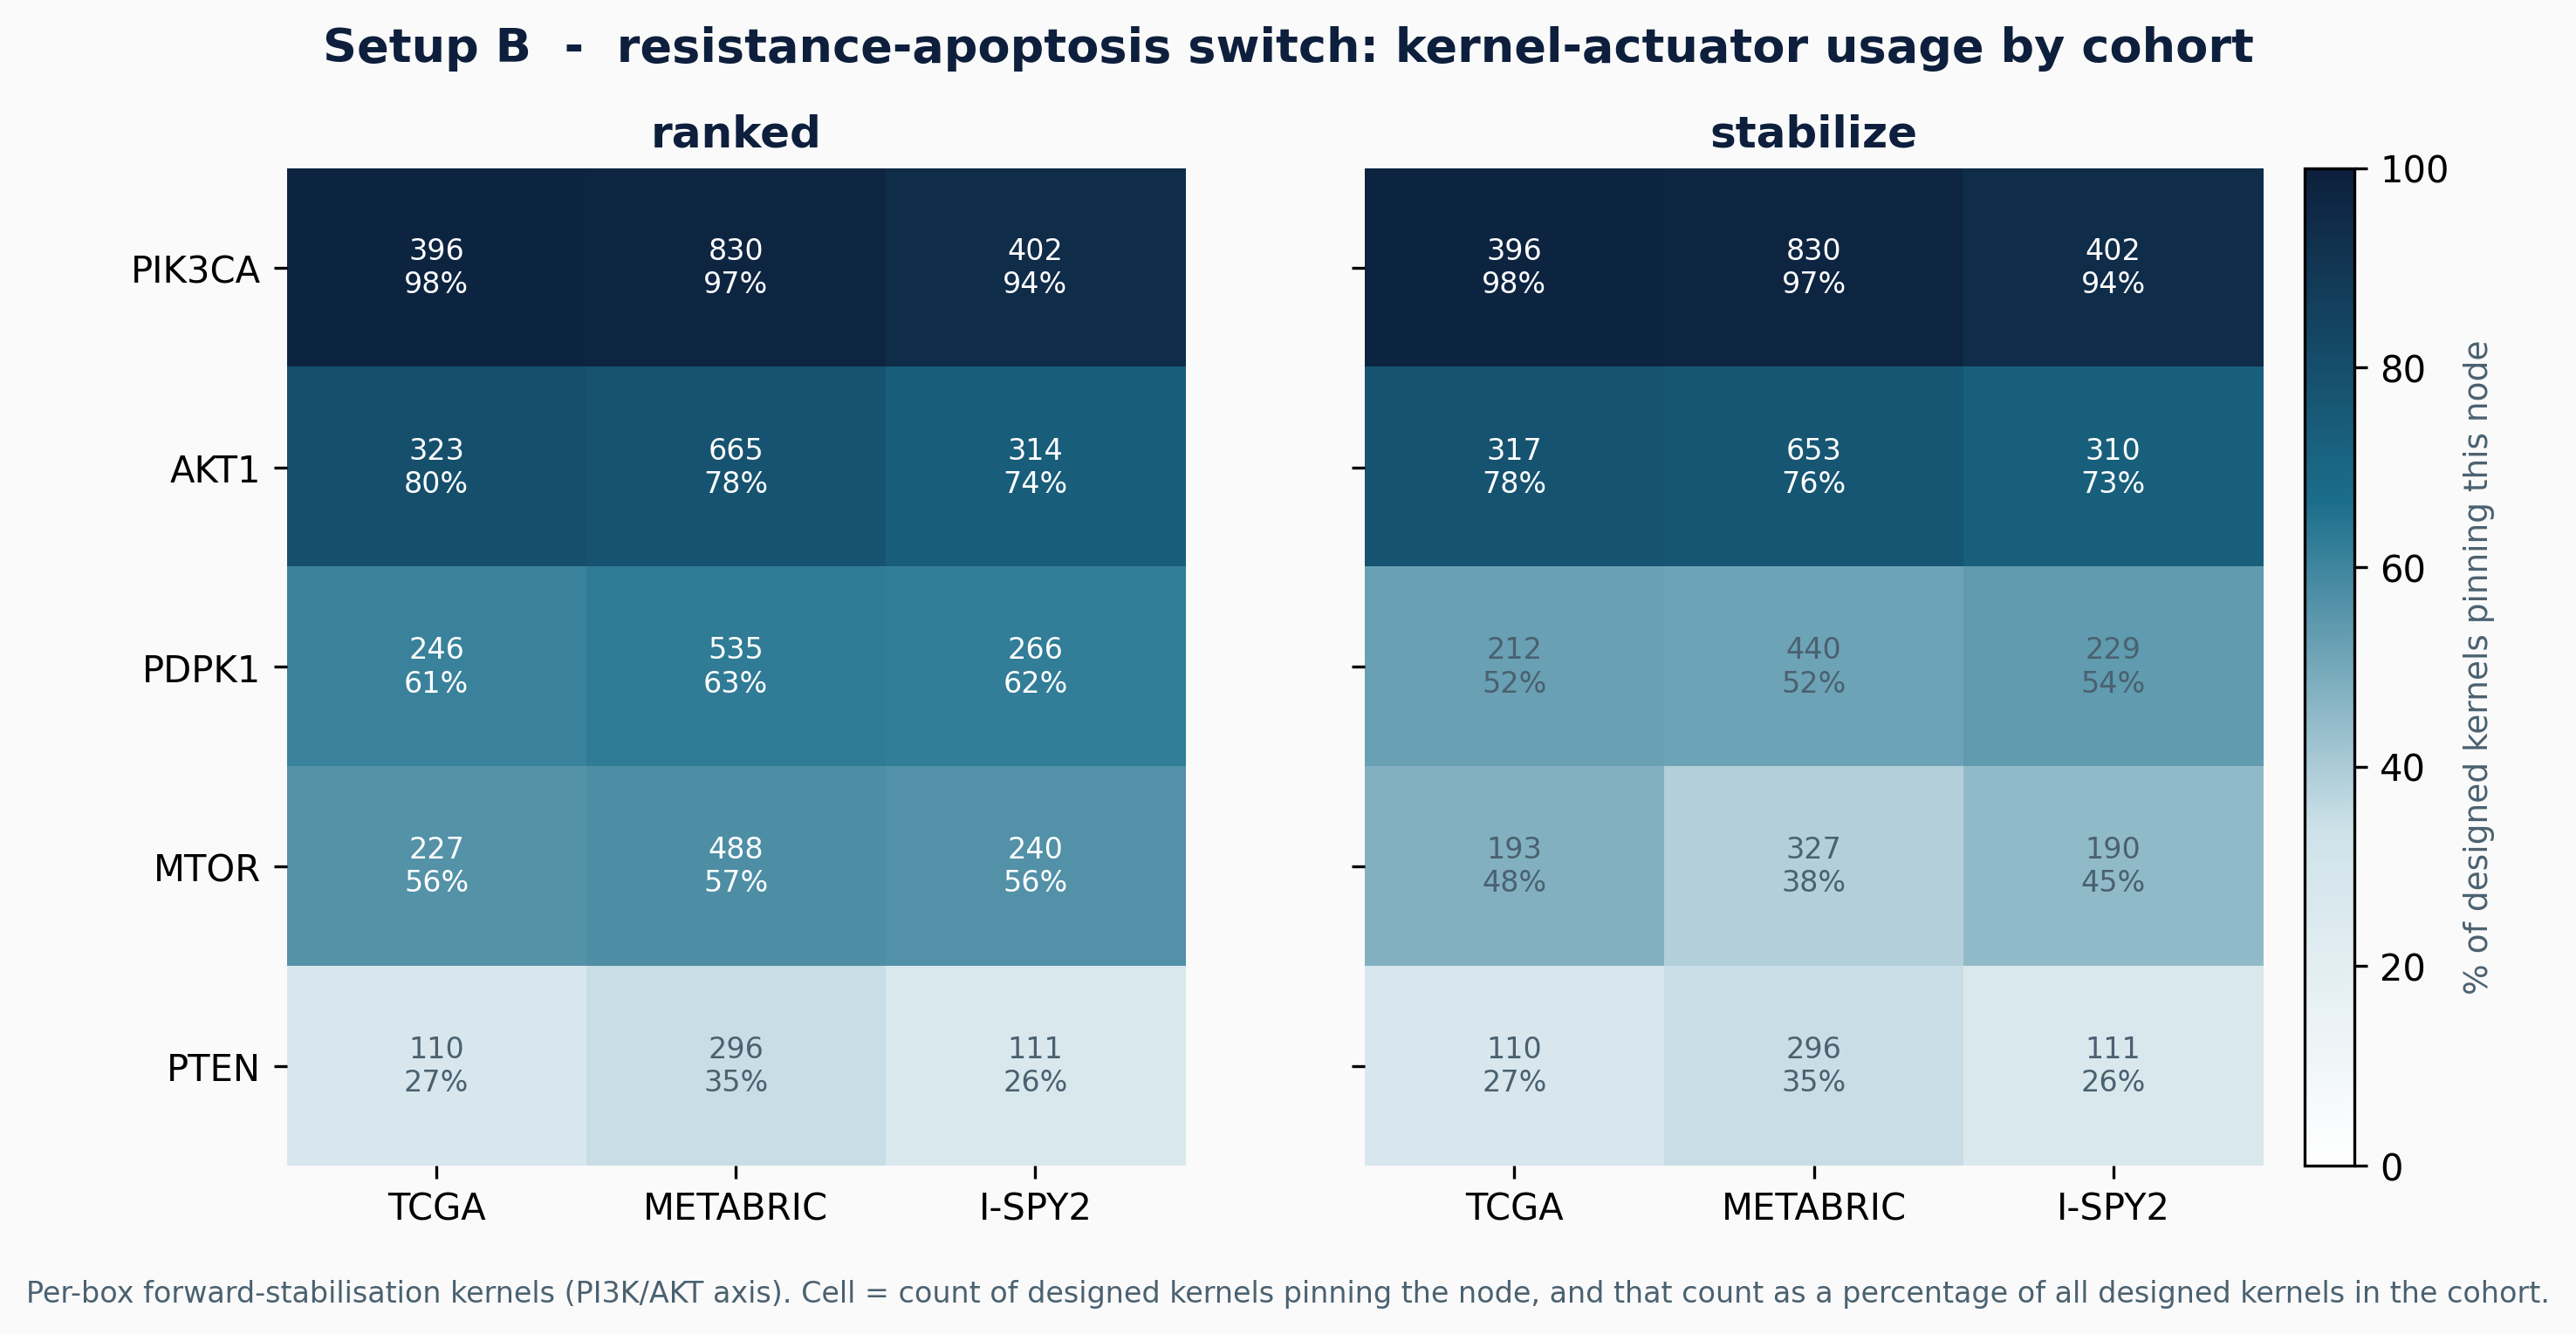
\includegraphics[width=\textwidth]{figures/figB_kernel_actuator.png}
\caption{\textbf{Setup~B kernel actuators: the PI3K/AKT/mTOR nomination.} For each cohort, the per-box forward-stabilisation kernels that flip resistant patients toward apoptosis are tallied by node, under the ranked heuristic (left) and the algebraic global-stabilisation test (right). Each cell gives the count of designed kernels that pin the node, and that count as a percentage of all designed kernels in the cohort. PIK3CA is pinned in almost every kernel (94--98\%), followed by AKT1 (73--80\%) and the PDPK1/MTOR nodes, with PTEN least used. The ordering is the same across all three cohorts and is essentially identical between the two methods, so the drug-target nomination is robust to both the cohort and the kernel-selection criterion. Counts are computed from the same pipeline that emits the flip rates reported in the Supplement (Table~S1).}
\label{fig:kernelB}
\end{figure}

This routing and its resistance signature are not an artefact of receptor-positive disease. On the same receptor-low (TNBC-like) subset, the switch routes patients in proportions close to the full cohort, and the survival-routed cells remain almost entirely in the uncoupled resistant state (Figure~\ref{fig:tnbcB}). The hysteresis reading of residual resistance therefore holds across receptor subtypes.

\begin{figure}[h]
\centering
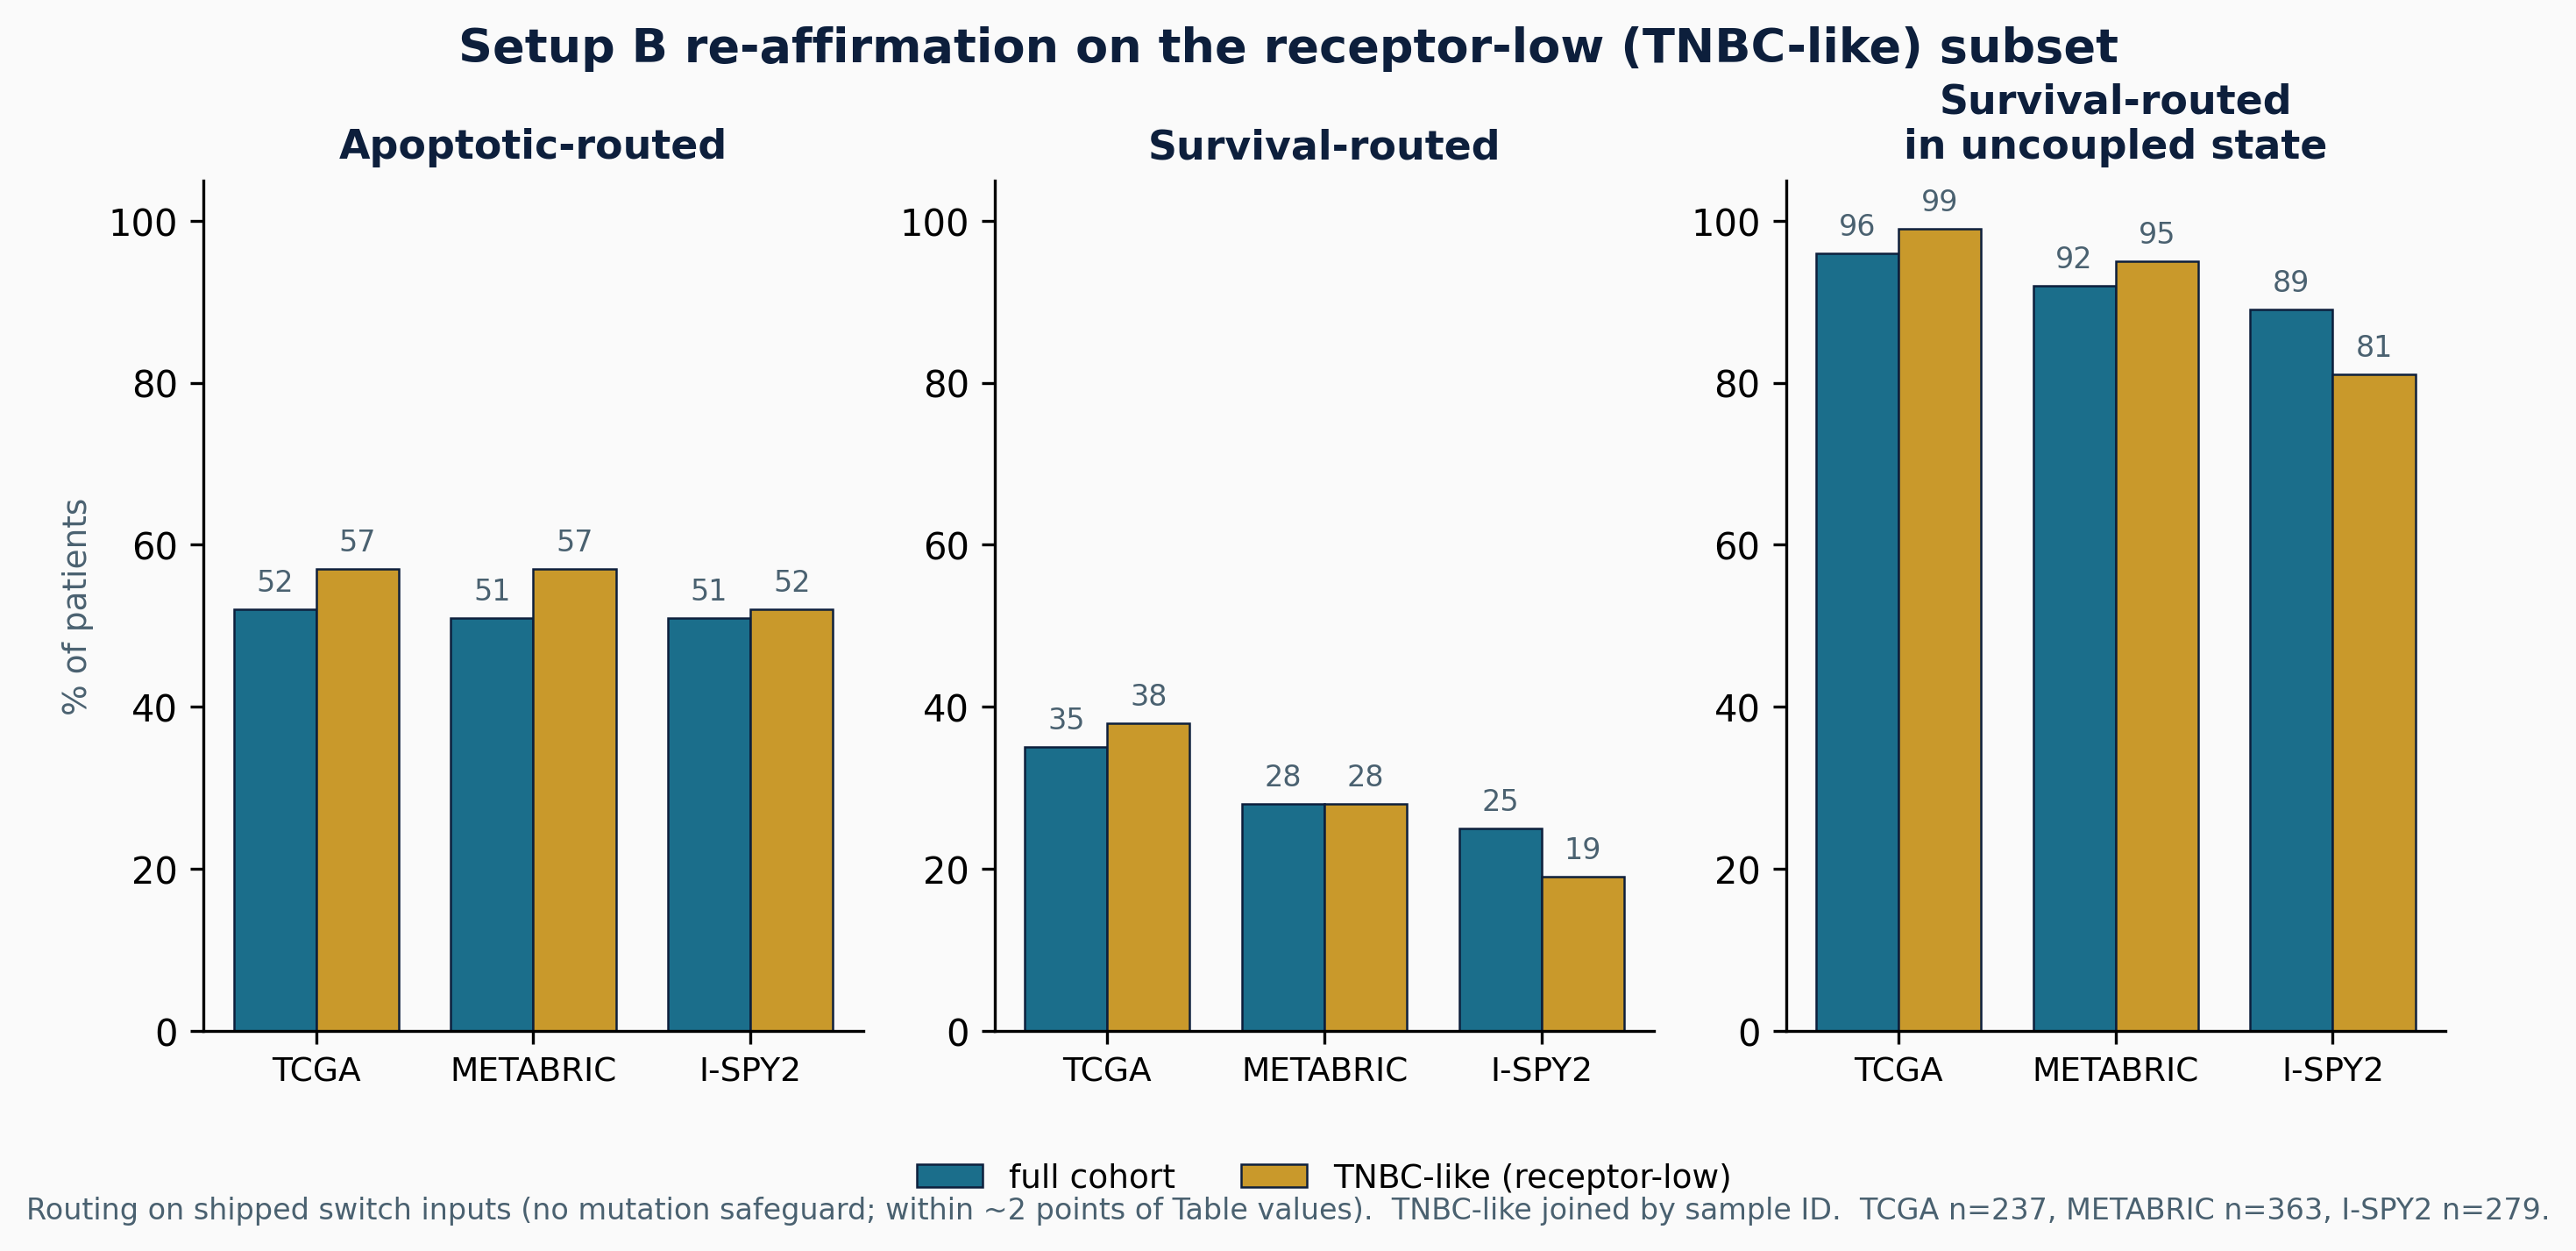
\includegraphics[width=\textwidth]{figures/figB_tnbc_panel.png}
\caption{\textbf{Setup B routing re-affirmed on the receptor-low (TNBC-like) subset.} Switch routing (apoptotic, survival) and the survival-routed uncoupled rate, for the full cohort (teal) and the receptor-low subset (gold). Routing here is computed on the shipped switch inputs without the mutation safeguard, so the percentages sit within about two points of the Table~\ref{tab:setupB} values; the within-cohort full-versus-subset comparison uses the same method throughout. The survival-routed uncoupled enrichment, which is the structural basis of the hysteresis reading, holds in the subset.}
\label{fig:tnbcB}
\end{figure}

\subsection{The repair recovers durable, controllable apoptosis}
\label{sec:repair}
The three repairs of Section~\ref{sec:repairs} change the network's behaviour, and the change is the central result of this paper. Each finding holds patient by patient and across all three cohorts on the biology-faithful delayed network.

\emph{Drug resistance equals AKT--FOXO3a uncoupling.} Run at full $N$ on every patient, survival-axis inhibition durably flips exactly the coupled fraction of patients (\BBCNRepairDrugFlipRange\%) while every uncoupled patient resists. The equivalence between the drug-resistant phenotype and the uncoupled flag holds for \BBCNRepairResistUncouplingMatch\ of \BBCNRepairResistUncouplingTotal\ patients, \BBCNRepairResistUncouplingPct\%. Genotoxic input alone barely moves the resistant state (\BBCNRepairGenotoxicRange\%), so reversing resistance is a matter of restoring coupling, not of adding damage. This upgrades the baseline-switch prognostic alignment of Section~\ref{sec:34} to a deterministic equivalence, and it reverses the baseline reading that only genotoxic input can flip the resistant attractor. The uncoupling that defines resistance here is itself an established mechanism~\cite{brunet1999,chen2010}; the contribution is to recover it as a clean deterministic equivalence across the full cohort and make it a control target.

\emph{A single designed kernel commits most resistant cells.} A minimal druggable kernel designed on the tractable switch by forward stabilisation, restricted to druggable nodes, is found for \BBCNRepairKernelFoundRange\% of resistant patients and concentrates on the PI3K/AKT/mTOR axis, the same nomination as the baseline-network analysis (Figure~\ref{fig:kernelB}). Tested on the full 136-node biology-faithful network, the designed clamp commits \BBCNRepairCommitRange\% of resistant patients to apoptosis. The switch design and the full-network test agree once death is scored by caspase commitment rather than by sustained survival-signal suppression.

\emph{The staged controller recovers durable fixed points.} Re-running the literal three-tier controller on the biology-faithful branch, apoptosis is controllable in \BBCNRepairApoptosisRange\% of patients and proliferation in \BBCNRepairProliferationRange\%, all three stages jointly in \BBCNRepairJointRange\% (against 2--3\% baseline), and, decisively, the network now settles into durable apoptotic fixed points in \BBCNRepairDurableRange\% of patients where the baseline network supported none (Table~\ref{tab:repair}).

\emph{Two honest readouts.} We score death two ways. The strict readout requires the executioner caspase on and the survival kinase stably off; it reads \BBCNRepairStrictRange\%. The commitment readout requires sustained caspase-3 activation, the irreversible point of no return, and reads \BBCNRepairCommitRange\%. The two differ because in uncoupled cells the survival kinase reactivates after withdrawal, so the strict readout records a survivor even though the cell has already committed to death; a committed cell does not un-die when a kinase switches back on. The two numbers answer different questions and we report both; both stand far above the baseline network's zero.

\begin{table}[h]
\centering
\begin{tabular}{lrrrrr}
\hline
Cohort & Resistant & Kernel commit & Durable FP & Apoptosis & Proliferation \\
\hline
TCGA     & \BBCNRepairTcgaResistantPct\%     & \BBCNRepairTcgaFullnetCommitPct\%     & \BBCNRepairTcgaDurablePct\%     & \BBCNRepairTcgaApoptosisPct\%     & \BBCNRepairTcgaProliferationPct\%     \\
METABRIC & \BBCNRepairMetabricResistantPct\% & \BBCNRepairMetabricFullnetCommitPct\% & \BBCNRepairMetabricDurablePct\% & \BBCNRepairMetabricApoptosisPct\% & \BBCNRepairMetabricProliferationPct\% \\
I-SPY2   & \BBCNRepairIspyTwoResistantPct\%   & \BBCNRepairIspyTwoFullnetCommitPct\%   & \BBCNRepairIspyTwoDurablePct\%   & \BBCNRepairIspyTwoApoptosisPct\%   & \BBCNRepairIspyTwoProliferationPct\%   \\
Baseline & --- & --- & 0\% & 81--86\% & 94--95\% \\
\hline
\end{tabular}
\caption{\textbf{The biology-faithful network, all three cohorts.} Drug-resistance equals AKT--FOXO3a uncoupling for \BBCNRepairResistUncouplingPct\% of \BBCNRepairResistUncouplingTotal\ patients. A designed PI3K/AKT/mTOR kernel commits \BBCNRepairCommitRange\% of resistant patients to apoptosis (commitment readout). The staged controller recovers durable apoptotic fixed points (\BBCNRepairDurableRange\%) absent from the baseline network. All values are macro-sourced from \texttt{numbers2.tex}; resistance, kernel, and durability are full-$N$ runs, with the staged-controller figures re-verified on a per-cohort sample.}
\label{tab:repair}
\end{table}

% ===== Paper 4 addition: minimality + release-and-persist durability =====
\subsection{\texorpdfstring{\new{A minimal kernel holds the apoptotic state that whole-network control also holds}}{A minimal kernel holds the apoptotic state that whole-network control also holds}}
\label{sec:minimality}
\new{The durable apoptosis recovered above can be secured by a far smaller intervention than the whole-network controller needs. Running both control designs through the same delayed engine and the same release-and-persist readout, and scoring durability as persistence of the death state after every kernel node is unpinned, death is reached in \HeldPct\% of patients under either design; what separates them is whether it persists. A minimal switch kernel holds the apoptotic state about as well as the near whole-network controller (switch durability \SwitchDurTcga/\SwitchDurMet/\SwitchDurIspy\% versus \WNDurTcga/\WNDurMet/\WNDurIspy\% for TCGA/METABRIC/I-SPY2), while being an order of magnitude smaller (about \SwitchSizeTcga\ versus about \WNSizeTcga\ nodes, a roughly \SizeRatio-fold reduction (12--13-fold across the three cohorts); Figure~\ref{fig:durability}, Table~\ref{tab:minimality}). The contribution is minimality at equal durability: the switch holds the same durable state with a focused, druggable kernel where the whole-network controller needs near whole-network control that is not a deliverable regimen. Across the three cohorts \KerneledTotal\ resistant patients receive a designed switch kernel (\KerTcga+\KerMet+\KerIspy).}

\begin{figure}[H]\centering

\includegraphics[width=\textwidth]{figures/f06_durability.pdf}
\caption{\new{\textbf{A minimal switch kernel secures the same durable apoptotic state as near whole-network control.} (A) Mean kernel size, about \SwitchSizeTcga\ nodes for the switch versus about \WNSizeTcga\ for the whole-network controller, a roughly \SizeRatio-fold reduction (12--13-fold across cohorts). (B) Durability after kernel withdrawal is essentially equal, with death reached in \HeldPct\% of patients either way. Regenerated by \texttt{fig6.py} from \texttt{setup\_a/data/cde\_vs\_switch\_summary.csv}.}}
\label{fig:durability}
\end{figure}

\begin{table}[H]\centering
\caption{\new{Durability and kernel size, switch versus whole-network controller (release-and-persist test on the switch-routed resistant set). Source: \texttt{cde\_vs\_switch\_summary.csv}.}}
\label{tab:minimality}
\begin{tabular}{lccc}
\toprule
Quantity & TCGA & METABRIC & I-SPY2 \\
\midrule
Resistant (switch-routed) & \ResSwitchTcga & \ResSwitchMet & \ResSwitchIspy \\
Kerneled (design found) & \KerTcga & \KerMet & \KerIspy \\
Death reached (held) \% & \HeldPct & \HeldPct & \HeldPct \\
Switch durability \% & \SwitchDurTcga & \SwitchDurMet & \SwitchDurIspy \\
Whole-network durability \% & \WNDurTcga & \WNDurMet & \WNDurIspy \\
Switch kernel size (nodes) & \SwitchSizeTcga & \SwitchSizeMet & \SwitchSizeIspy \\
Whole-network size (nodes) & \WNSizeTcga & \WNSizeMet & \WNSizeIspy \\
\bottomrule
\end{tabular}
\end{table}

\new{Durability rests on the intact coupling. With PHLPP intact the kerneled state is durable and AKT stays off after release.} \new{This is the apoptotic-side counterpart of the resistant-side hysteresis in Section~\ref{sec:34}: the same coupling whose loss defines resistance is what makes induced death durable, consistent with the deterministic equivalence of resistance and AKT--FOXO3a uncoupling (\BBCNRepairResistUncouplingMatch\ of \BBCNRepairResistUncouplingTotal\ patients, \BBCNRepairResistUncouplingPct\%).}

\new{The designed kernels map to a small druggable set and independently nominate the PI3K/\allowbreak AKT/\allowbreak mTOR axis, overlapping the I-SPY2 AKT-inhibitor arm~\cite{turner2023}. The full kernel-to-drug nomination, ranked by Hamming descent, is given in Table~\ref{tab:drugs}.}

\begin{table}[H]\centering\footnotesize
\caption{\new{Kernel-to-drug nominations across the pathway set (source: \texttt{bbcn/drugs.py}).}}
\label{tab:drugs}
\setlength{\tabcolsep}{4pt}\begin{tabular}{@{}p{2.2cm}p{2.9cm}p{2.5cm}p{3.2cm}p{1.7cm}@{}}
\toprule
Pathway & Kernel target & Drug class & Lead agent (alternatives) & Approval \\
\midrule
Apoptosis intrinsic & BAX, CYCS, APAF1 on & BCL-2 family inhibitor & Venetoclax (Navitoclax) & FDA approved \\
MAPK & MAP2K1, RAF1, MAPK1 off & MEK + RAF inhibitor & Trametinib (Dabrafenib) & FDA approved \\
Cell cycle & CCND1, E2F1 off; RB1 on & CDK4/6 inhibitor & Palbociclib (Ribociclib) & FDA approved \\
MYC / TF & MYC off; CDKN2A, RB1 on & BET inhibitor & Molibresib (ZEN-3694) & Phase I/II \\
AKT survival & TP53 on; XIAP, CFLAR off & MDM2i + IAP antagonist & Idasanutlin (Birinapant) & Phase I/II \\
AKT signaling & AKT1 off; FOXO3 on & AKT inhibitor & Ipatasertib (Capivasertib) & Phase II/III \\
JAK / STAT & JAK2, STAT3 off & JAK1/2 inhibitor & Ruxolitinib (Fedratinib) & FDA approved \\
Apoptosis regulatory & MCL1 off; CASP9 on & MCL1 inhibitor & S63845 (AZD5991) & Phase I \\
CDK cell cycle & CDK4, CDK6 off & CDK4/6 inhibitor & Abemaciclib (Palbociclib) & FDA approved \\
Apoptosis extrinsic & CASP3, CASP9 on & TRAIL receptor agonist & Dulanermin (Tigatuzumab) & Phase I/II \\
PI3K & PTEN on & PI3K inhibitor & Alpelisib (Copanlisib) & FDA approved \\
NF-kB & RELA off & NF-kB / proteasome inhibitor & Bortezomib (Ixazomib) & FDA approved \\
\bottomrule
\end{tabular}
\end{table}

\subsection{Validation, and the limits of prediction}
\label{sec:35}
The nominated targets are real: the kernel genes (PIK3CA, AKT1, MTOR) are established, mostly-approved breast-cancer drug targets in curated drug-target evidence, and this concordance is robust across all three input front-ends (median-binarised expression, multi-gene signatures, and phospho-protein activity). Mutation concordance is weaker (METABRIC $p\approx0.02$; TCGA not significant), as expected when the model reads pathway activity rather than genotype. The model does not predict pathologic complete response: on the I-SPY2 AKT-inhibitor arm the routing is not concordant with pCR, and we ruled out two explanations, binarisation (continuous and binarised inputs are equally flat) and expression-versus-signalling (phospho-seeded inputs fail at pCR too). The remaining explanation is endpoint distance: pCR is a distal, whole-tumour outcome shaped by immune, stromal, and pharmacokinetic factors beyond the single-cell decision the switch models. The defensible role of the model is a structural stratifier and drug-target nominator, not a response predictor.
\authornote{survival-association and cell-line concordance to be reconciled to the current model version before inclusion; the public-repo position is an explicit null on survival benefit, stated honestly.}

\subsection{The two kernel methods compared}
\label{sec:comparison}
The two kernel-design methods, the ranked reachability heuristic and the algebraic global-stabilisation test, were compared on the baseline 135-node network under synchronous updating (Setup~A of Sections~3.1--3.2), to isolate the kernel method from the biological repairs. They agree across all three cohorts: the ranked method reproduces the earlier BBCN118 kernels exactly, and the algebraic test is the conservative, provable bound, certifying fewer passes only where a favourable initial state, rather than global stabilisability, carried the heuristic. In the figures the algebraic method is labelled \emph{stabilize} and the heuristic \emph{ranked}; these are two names for the same kernel-selection step. The full per-phenotype comparison (Table~S1) and the kernel-usage breakdown (Figure~S1) are given in the Supplement.

% ------------------------------------------------------------
\section{Discussion}
Two findings carry the work. First, cell-fate phenotypes in this network are individually controllable but jointly near-exclusive, because they share a dominant strongly-connected core; feasibility does not imply reachability, and pathway-by-pathway control fails on the core. This complements stable-motif and STP control theory, which establish when a target attractor is controllable, by showing that under a realistic capped budget on real patient states the binding constraint is joint reachability across coupled phenotypes. Second, the hardest phenotype is best understood not as a target to push but as one attractor of a bistable resistance--apoptosis switch, and flipping it requires crossing a hysteresis barrier that survival-axis inhibition alone cannot cross. Embedding biological timescale separation as a delayed (autoregressive) multirate structure is what makes the core controllable where the whole-network controller could not; to our knowledge this direct embedding of timescale separation in the control of a patient-specific Boolean cancer model is novel.

A third finding reframes the first two. The baseline network's non-durability, and its reading that only genotoxic input can flip the resistant attractor, are substantially artifacts of wiring rather than statements about the biology. Three collapsed feedback loops, a degenerate p53 sensor, an unclosed AKT--FOXO arm, and the absence of an irreversible commitment step, are enough to abolish durable apoptosis and to make the survival axis look untouchable. Restoring each to its textbook form, with no tuning, turns the obstruction into durable, controllable apoptosis: drug resistance becomes the precise molecular state of AKT--FOXO3a uncoupling, an established resistance mechanism~\cite{brunet1999,chen2010} that the model recovers as a deterministic equivalence, a single designed PI3K/AKT/mTOR kernel commits about nine in ten resistant cells to death, and the staged controller recovers durable apoptotic fixed points the baseline network lacked. The two levers are co-equal and do different jobs: the biological repairs make the durable death state exist as a genuine fixed point, while the timescale separation of Setup~B makes it reachable and stable under realistic dynamics. The reduced switch and the full network agree once death is scored as commitment. The baseline-network results above are not retracted; they are the correct behaviour of the uncorrected wiring, and the contrast between them and the biology-faithful network is the contribution.

The validated outputs are a coherent patient stratification and a robust PI3K/AKT/mTOR drug-target nomination independent of input front-end. The honest limit is that the model does not predict pathologic complete response, which we attribute to endpoint distance rather than signal quality. The framework is a mechanistic hypothesis generator and structural stratifier; clinical benefit is not demonstrated here.
\authornote{limitations (proxy $U$ flag; invasion out of scope; primary tumours only; binary modelling choice) and the road to clinical testing to be expanded at prose stage.}

% ------------------------------------------------------------
\new{A natural objection is that durability may not matter if a drug is simply never withdrawn. It does matter. Continuous inhibition is itself what breeds resistance, because sustained blockade relieves the pathway's own feedback and the target reactivates~\cite{chandarlapaty2011}; a state held only by constant force collapses at every missed dose, whereas a durable one inside the death basin survives them; whole-network control across about thirty nodes is lifelong polypharmacy and not tolerable, so minimality is what makes any maintenance conceivable; and apoptosis is terminal, so a cell that durably commits needs no further dosing. The bistable-caspase lineage that grounds this commitment picture is developed by Eissing and colleagues, Legewie and colleagues, and Bagci and colleagues~\cite{eissing2004,legewie2006,bagci2006}, with single-cell apoptosis dynamics quantified by Albeck and colleagues~\cite{albeck2008}, and the control-kernel and feedback-vertex-set view by Kim, Park and Cho and by Fiedler and colleagues~\cite{kimparkcho2013,fiedler2013}. The delayed Boolean control formalism follows Li and Sun, Lu and colleagues, and Parmar and colleagues~\cite{lisun2011,lu2016,parmar2015}.}

\new{The step that would most raise the translational ceiling is a durability-matched validation: because durability corresponds to relapse-avoidance, the direct external test is whether AKT--FOXO3a coupling status, read from expression, stratifies relapse-free or overall survival in a long-follow-up cohort such as METABRIC. That test should be run against the current model and reported at face value, whichever way it lands.}

\section*{Code and data availability}
All numbers, figures, and tables regenerate from the companion repository
(\url{https://github.com/AamerIqbalBhatti/Systems_Biology_Journal_2026}) with a single command (\texttt{python reproduce\_all.py}); Cohort inputs: TCGA-BRCA is open access and its binarised inputs are shipped with the code, so the pipeline runs out of the box on that cohort. METABRIC is available under controlled access through the European Genome-phenome Archive (processed data via cBioPortal under its data-use terms), and I-SPY2 expression is available from Gene Expression Omnibus series GSE194040; to comply with those terms the patient-level matrices for these two cohorts are not redistributed, but the deterministic binarisation procedure is specified in Section~\ref{sec:cohorts}, so a user with the primary data regenerates the inputs and reproduces every result. One-click reproduction of the shipped-cohort figures is also provided via Google Colab and Binder.

\section*{Declaration of generative AI use}
During the preparation of this manuscript the author used a large language model (Anthropic's Claude) as an assistive tool for \LaTeX{} formatting and typesetting, for writing figure-generation code, for organising the companion code repository, and for language editing and drafting assistance on author-directed text. The tool was not used to generate scientific content, data, analyses, results, or their interpretation, and it is not an author. The author directed all such use, verified every reported number against the source code, and takes full responsibility for the entire content of the manuscript.

% ------------------------------------------------------------
\appendix
% AUTO-GENERATED by generate_rules_appendix.py from setup_a/bbcn/pathways.py -- DO NOT EDIT BY HAND.
\section{The BBCN digital logic model}
\label{app:rules}
This appendix lists the complete Boolean update logic of the BBCN network, one block per pathway module, generated directly from the source file \texttt{pathways.py} so that the printed rules cannot drift from the code. For each node, the right-hand side is its update rule over intra-pathway nodes and external bus inputs; \texttt{AND}, \texttt{OR}, \texttt{NOT} are the Boolean connectives. A node with rule equal to a single input is a pass-through of that input.

\paragraph{RTK EGFR. (Upstream\_RTK)}\mbox{}\\
\begin{flushleft}\ttfamily\small
EGF = EGF\\
EGFR = (EGF OR (ERBB2 AND ERBB3)) AND NOT MAP2K1\\
GRB2 = IRS1 OR (LATS1 OR (EGFR OR SRC))\\
GRB7 = GRB7 AND NOT PRKACA\\
ERBB2 = ERBB3 OR EGF\\
ERBB3 = NRG1 OR ERBB2\\
\end{flushleft}

\paragraph{RTK INSULIN. (Upstream\_RTK)}\mbox{}\\
\begin{flushleft}\ttfamily\small
INS = INS\\
INSR = INS OR FOXO3\\
IRS1 = NOT RPS6KB1 AND (INSR OR IGF1R)\\
PIK3CA = GRB2 OR IRS1\\
ABL1 = GRB2 OR EGFR OR ERBB2 OR IRS1\\
\end{flushleft}

\paragraph{HORMONE. (Upstream\_Hormone)}\mbox{}\\
\begin{flushleft}\ttfamily\small
AR = FOXO3 OR NOT AKT1\\
PGR = ESR1\\
ESR1 = (FOXO3 OR KMT2D) AND NOT AKT1\\
KMT2D = PAX7\\
\end{flushleft}

\paragraph{PI3K. (Terminal\_support)}\mbox{}\\
\begin{flushleft}\ttfamily\small
PTEN = NOT SRC\\
PDPK1 = (PIK3CA AND NOT PTEN) OR IGF1R\\
RAC1 = (PIK3CA OR DVL1) AND NOT AKT1\\
NOS3 = HSP90AA1 OR AKT1\\
\end{flushleft}

\paragraph{MAPK. (Resistance)}\mbox{}\\
\begin{flushleft}\ttfamily\small
HRAS = SOS1 AND NOT NF1\\
MAP2K1 = RAF1\\
RAF1 = HRAS OR KRAS\\
KRAS = SOS1\\
SOS1 = GRB2\\
NF1 = (TP53 OR FOXO3) AND NOT (MAPK1 OR AKT1)\\
MAPK8 = (FAS OR TRADD) AND NOT (AKT1 OR MAPK1)\\
MAPK1 = MAP2K1 AND NOT DUSP1\\
DUSP1 = MAPK1 OR MAPK8 OR JUN\\
\end{flushleft}

\paragraph{WNT. (Invasion\_OFF)}\mbox{}\\
\begin{flushleft}\ttfamily\small
APC = AXIN1\\
AXIN1 = NOT DVL1 AND GSK3B\\
CTNNB1 = NOT (APC AND AXIN1 AND GSK3B) AND (WNT1 OR SRC OR YAP1)\\
DVL1 = FZD3 OR NF1\\
FZD3 = WNT1 OR CREB1\\
RND1 = GRB7 OR DVL1\\
TCF7L2 = CTNNB1 OR JUN\\
WNT1 = WNT1\\
\end{flushleft}

\paragraph{NOTCH. (Invasion\_OFF)}\mbox{}\\
\begin{flushleft}\ttfamily\small
ABL2 = ABL1\\
DLL1 = DLL1\\
HES1 = NOTCH1\\
HEY1 = NOTCH1\\
EIF4EBP1 = NOT MTOR\\
MYOD1 = NOT (HES1 OR ABL1)\\
MYOG = NOT HEY1 AND MYOD1\\
NOTCH1 = DLL1 OR CTNNB1 OR LCK OR MDM2\\
\end{flushleft}

\paragraph{JAK STAT. (Xglobal\_Tier1)}\mbox{}\\
\begin{flushleft}\ttfamily\small
JAK2 = IL6 AND IL6R\\
STAT3 = JAK2\\
STAT1 = JAK2 AND NOT AKT1\\
SOCS3 = STAT3 OR STAT1\\
\end{flushleft}

\paragraph{HIPPO. (Invasion\_OFF)}\mbox{}\\
\begin{flushleft}\ttfamily\small
YAP1 = NOT LATS1\\
LATS1 = NF2 OR LCK\\
NF2 = NEDD4L\\
\end{flushleft}

\paragraph{AKT SIGNALING. (Xglobal\_Tier1)}\mbox{}\\
\begin{flushleft}\ttfamily\small
AKT1 = (MTOR AND PDPK1) AND (PIK3CA AND NOT PTEN)\\
FOXO1 = NOT (SGK1 OR AKT1)\\
SGK1 = MTOR OR PDPK1\\
NEDD4L = NOT (SGK1 OR PRKACA)\\
FOXO3 = NOT AKT1\\
GSK3B = NOT (AKT1 OR MAPK1)\\
\end{flushleft}

\paragraph{MTOR. (Invasion\_OFF)}\mbox{}\\
\begin{flushleft}\ttfamily\small
RHEB = NOT TSC2\\
MTOR = RHEB OR (PIK3CA AND NOT PTEN)\\
TSC2 = NOT (AKT1 OR MAPK1) AND (PRKAA2 OR GSK3B)\\
TWIST1 = MAPK1 OR AKT1 OR MAPK8\\
\end{flushleft}

\paragraph{TF. (Xglobal\_Tier1)}\mbox{}\\
\begin{flushleft}\ttfamily\small
CEBPB = ABL2 OR CREB1\\
CREB1 = AKT1 AND NOT PTEN\\
EIF4E = NOT EIF4EBP1\\
GATA3 = NOT STAT1\\
CXCL8 = NOT GATA3\\
MYC = (CTNNB1 OR PIM1 OR PIM2 OR PIM3 OR MAPK1 OR STAT3 OR ESR1) AND NOT GSK3B\\
\end{flushleft}

\paragraph{NFKB. (Resistance\_OFF)}\mbox{}\\
\begin{flushleft}\ttfamily\small
IKBKB = TNF OR IL1A OR IL1B OR TLR2 OR TLR4 OR AKT1\\
NFKBIA = NOT IKBKB\\
RELA = IKBKB AND NOT NFKBIA\\
\end{flushleft}

\paragraph{INNATE IMMUNE. (Inflammatory)}\mbox{}\\
\begin{flushleft}\ttfamily\small
IL1A = IL1A\\
IL1B = IL1B\\
TLR2 = TLR2\\
TLR4 = TLR4\\
\end{flushleft}

\paragraph{AKT SURVIVAL. (Apoptosis\_ON)}\mbox{}\\
\begin{flushleft}\ttfamily\small
MDM2 = TP53 OR MDM2\\
TP53 = NOT MDM2\\
JUN = (MAPK8 OR MAPK1 OR RELA) AND NOT (PPARG OR DUSP1)\\
XIAP = AKT1 OR JUN\\
CFLAR = (AKT1 OR RELA OR CREB1) AND TP53\\
\end{flushleft}

\paragraph{APOPTOSIS REGULATORY. (Apoptosis\_ON)}\mbox{}\\
\begin{flushleft}\ttfamily\small
MCL1 = NOT GSK3B AND MAPK1\\
PAK1 = TCF7L2\\
PRKACA = AKT1 OR WNT1\\
SRC = PRKACA OR ABL1\\
\end{flushleft}

\paragraph{APOPTOSIS EXTRINSIC. (Xglobal\_Tier1)}\mbox{}\\
\begin{flushleft}\ttfamily\small
FAS = FASLG\\
FASLG = JUN OR RELA OR TP53\\
FADD = FAS OR TRADD\\
TRADD = FAS\\
CASP8 = FADD AND NOT CFLAR\\
BID = CASP8\\
CASP3 = (CASP8 OR CASP9) AND NOT XIAP\\
CASP9 = CYCS AND APAF1\\
\end{flushleft}

\paragraph{APOPTOSIS INTRINSIC. (Apoptosis\_ON)}\mbox{}\\
\begin{flushleft}\ttfamily\small
BAD = NOT (PAK1 OR AKT1 OR MAPK1 OR PIM1 OR PIM2 OR PIM3)\\
BAK1 = (BCL2L11 OR TP53 OR BCL2) AND NOT (MCL1 OR BCL2 OR BCL2L1)\\
BAX = (BCL2L11 OR TP53 OR BCL2) AND NOT (MCL1 OR BCL2 OR BCL2L1)\\
BCL2 = NOT (BAD OR BCL2L11) AND (CREB1 OR MAPK1)\\
BCL2L1 = NOT (BAD OR BCL2L11) AND CREB1\\
BCL2L11 = FOXO3 OR FOXO1\\
CYCS = BAK1 OR BAX\\
APAF1 = TP53 OR FOXO1 OR FOXO3\\
\end{flushleft}

\paragraph{CELLCYCLE. (Proliferation\_OFF)}\mbox{}\\
\begin{flushleft}\ttfamily\small
CDKN2A = NOT (MYC OR SRC OR AKT1 OR MAPK1)\\
CCND1 = (TCF7L2 OR TEAD1 OR MYC) AND NOT (CDKN2A OR CDKN1A OR GSK3B)\\
E2F1 = NOT RB1\\
CDKN1A = TP53 OR FOXO3 OR NOT (MAPK1 OR AKT1 OR MYC)\\
RB1 = NOT (CDK4 OR CDK6 OR CDK2 OR CCND1)\\
TEAD1 = YAP1\\
\end{flushleft}

\paragraph{CDK CELLCYCLE. (Proliferation\_OFF)}\mbox{}\\
\begin{flushleft}\ttfamily\small
CDK4 = CCND1 AND CDKN1B\\
CDK6 = CCND1 AND CDKN1B\\
CDK2 = CDK4 OR CDK6\\
CCNE1 = CDK4 OR CDK6\\
CDKN1B = FOXO1 OR FOXO3\\
\end{flushleft}

\paragraph{DNA REPAIR. (DNA\_Repair)}\mbox{}\\
\begin{flushleft}\ttfamily\small
ATM = ATM\\
ATR = ATR\\
BRCA1 = ATM OR ATR\\
BRCA2 = BRCA1\\
PARP1 = PARP1\\
CHEK1 = ATM\\
CHEK2 = ATR\\
RAD51 = BRCA1\\
\end{flushleft}

\paragraph{IMMUNE CHECKPOINT. (Immune\_Checkpoint)}\mbox{}\\
\begin{flushleft}\ttfamily\small
PDCD1 = LCK\\
CD274 = IFNG OR STAT3 OR AKT1\\
\end{flushleft}

\paragraph{AUX INPUTS1. (Boundary)}\mbox{}\\
\begin{flushleft}\ttfamily\small
HSP90AA1 = HSP90AA1  (external input)\\
IGF1R = IGF1R  (external input)\\
IL6 = IL6  (external input)\\
IL6R = IL6R  (external input)\\
LCK = LCK  (external input)\\
NRG1 = NRG1  (external input)\\
PAX7 = PAX7  (external input)\\
IFNG = IFNG  (external input)\\
\end{flushleft}

\paragraph{AUX INPUTS2. (Boundary)}\mbox{}\\
\begin{flushleft}\ttfamily\small
PIM1 = PIM1  (external input)\\
PIM2 = PIM2  (external input)\\
PIM3 = PIM3  (external input)\\
PPARG = PPARG  (external input)\\
PRKAA2 = PRKAA2  (external input)\\
RPS6KB1 = RPS6KB1  (external input)\\
TNF = TNF  (external input)\\
\end{flushleft}

\noindent\textit{Total: 135 nodes across 24 pathway modules.}

\section{Flowcharts of the two kernel-design methods}
\label{app:flow}
Both kernel methods take a pathway and its target state and return a minimal clamp set. They share the same candidate pool and the same size cap, and differ only in the acceptance criterion. The ranked heuristic accepts the patient-specific trajectory that reaches the target (Figure~\ref{fig:flowranked}); the algebraic test accepts only clamp sets that drive every pathway state to the target (Figure~\ref{fig:flowstab}).

\begin{figure}[H]
\centering
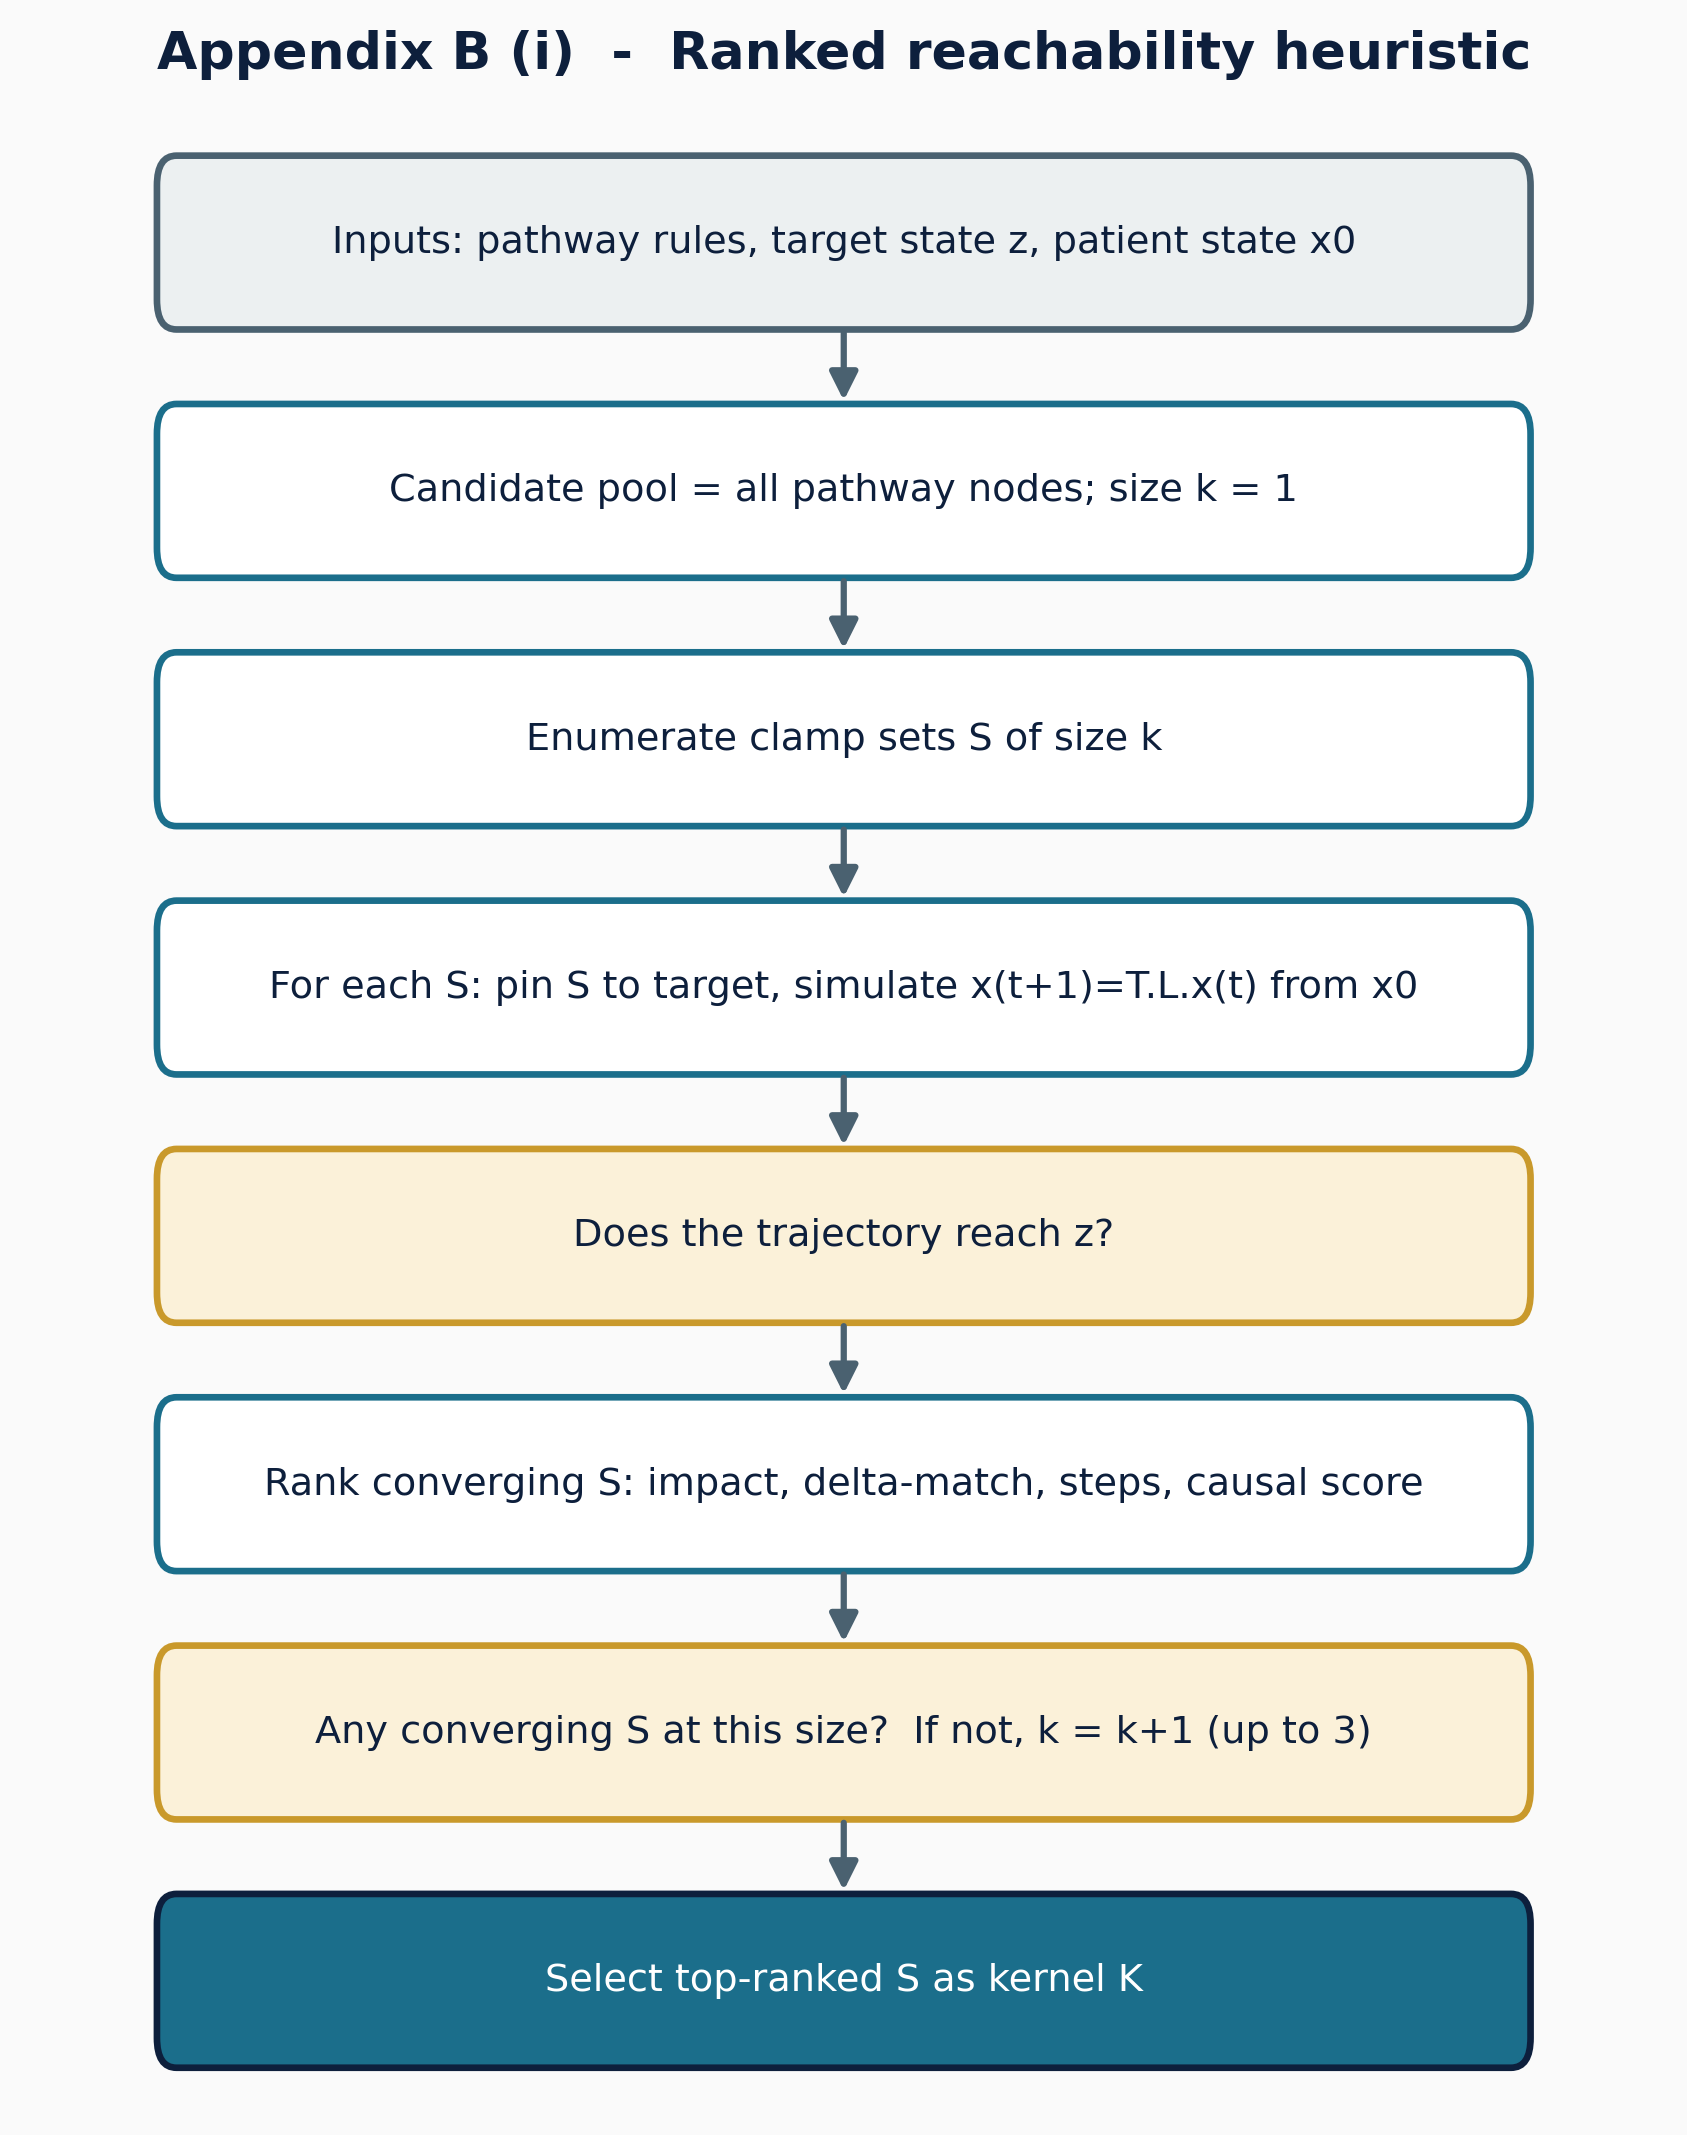
\includegraphics[width=0.6\textwidth]{figures/figC_flow_ranked.png}
\caption{\textbf{Ranked reachability heuristic (Tier~1).} Candidate clamp sets are enumerated by increasing size, each is simulated from the patient state, and converging sets are ranked by impact, then delta-match, then steps, then a causal score; the top set is the kernel. This is the heuristic that reproduces the earlier BBCN118 kernels.}
\label{fig:flowranked}
\end{figure}

\begin{figure}[H]
\centering
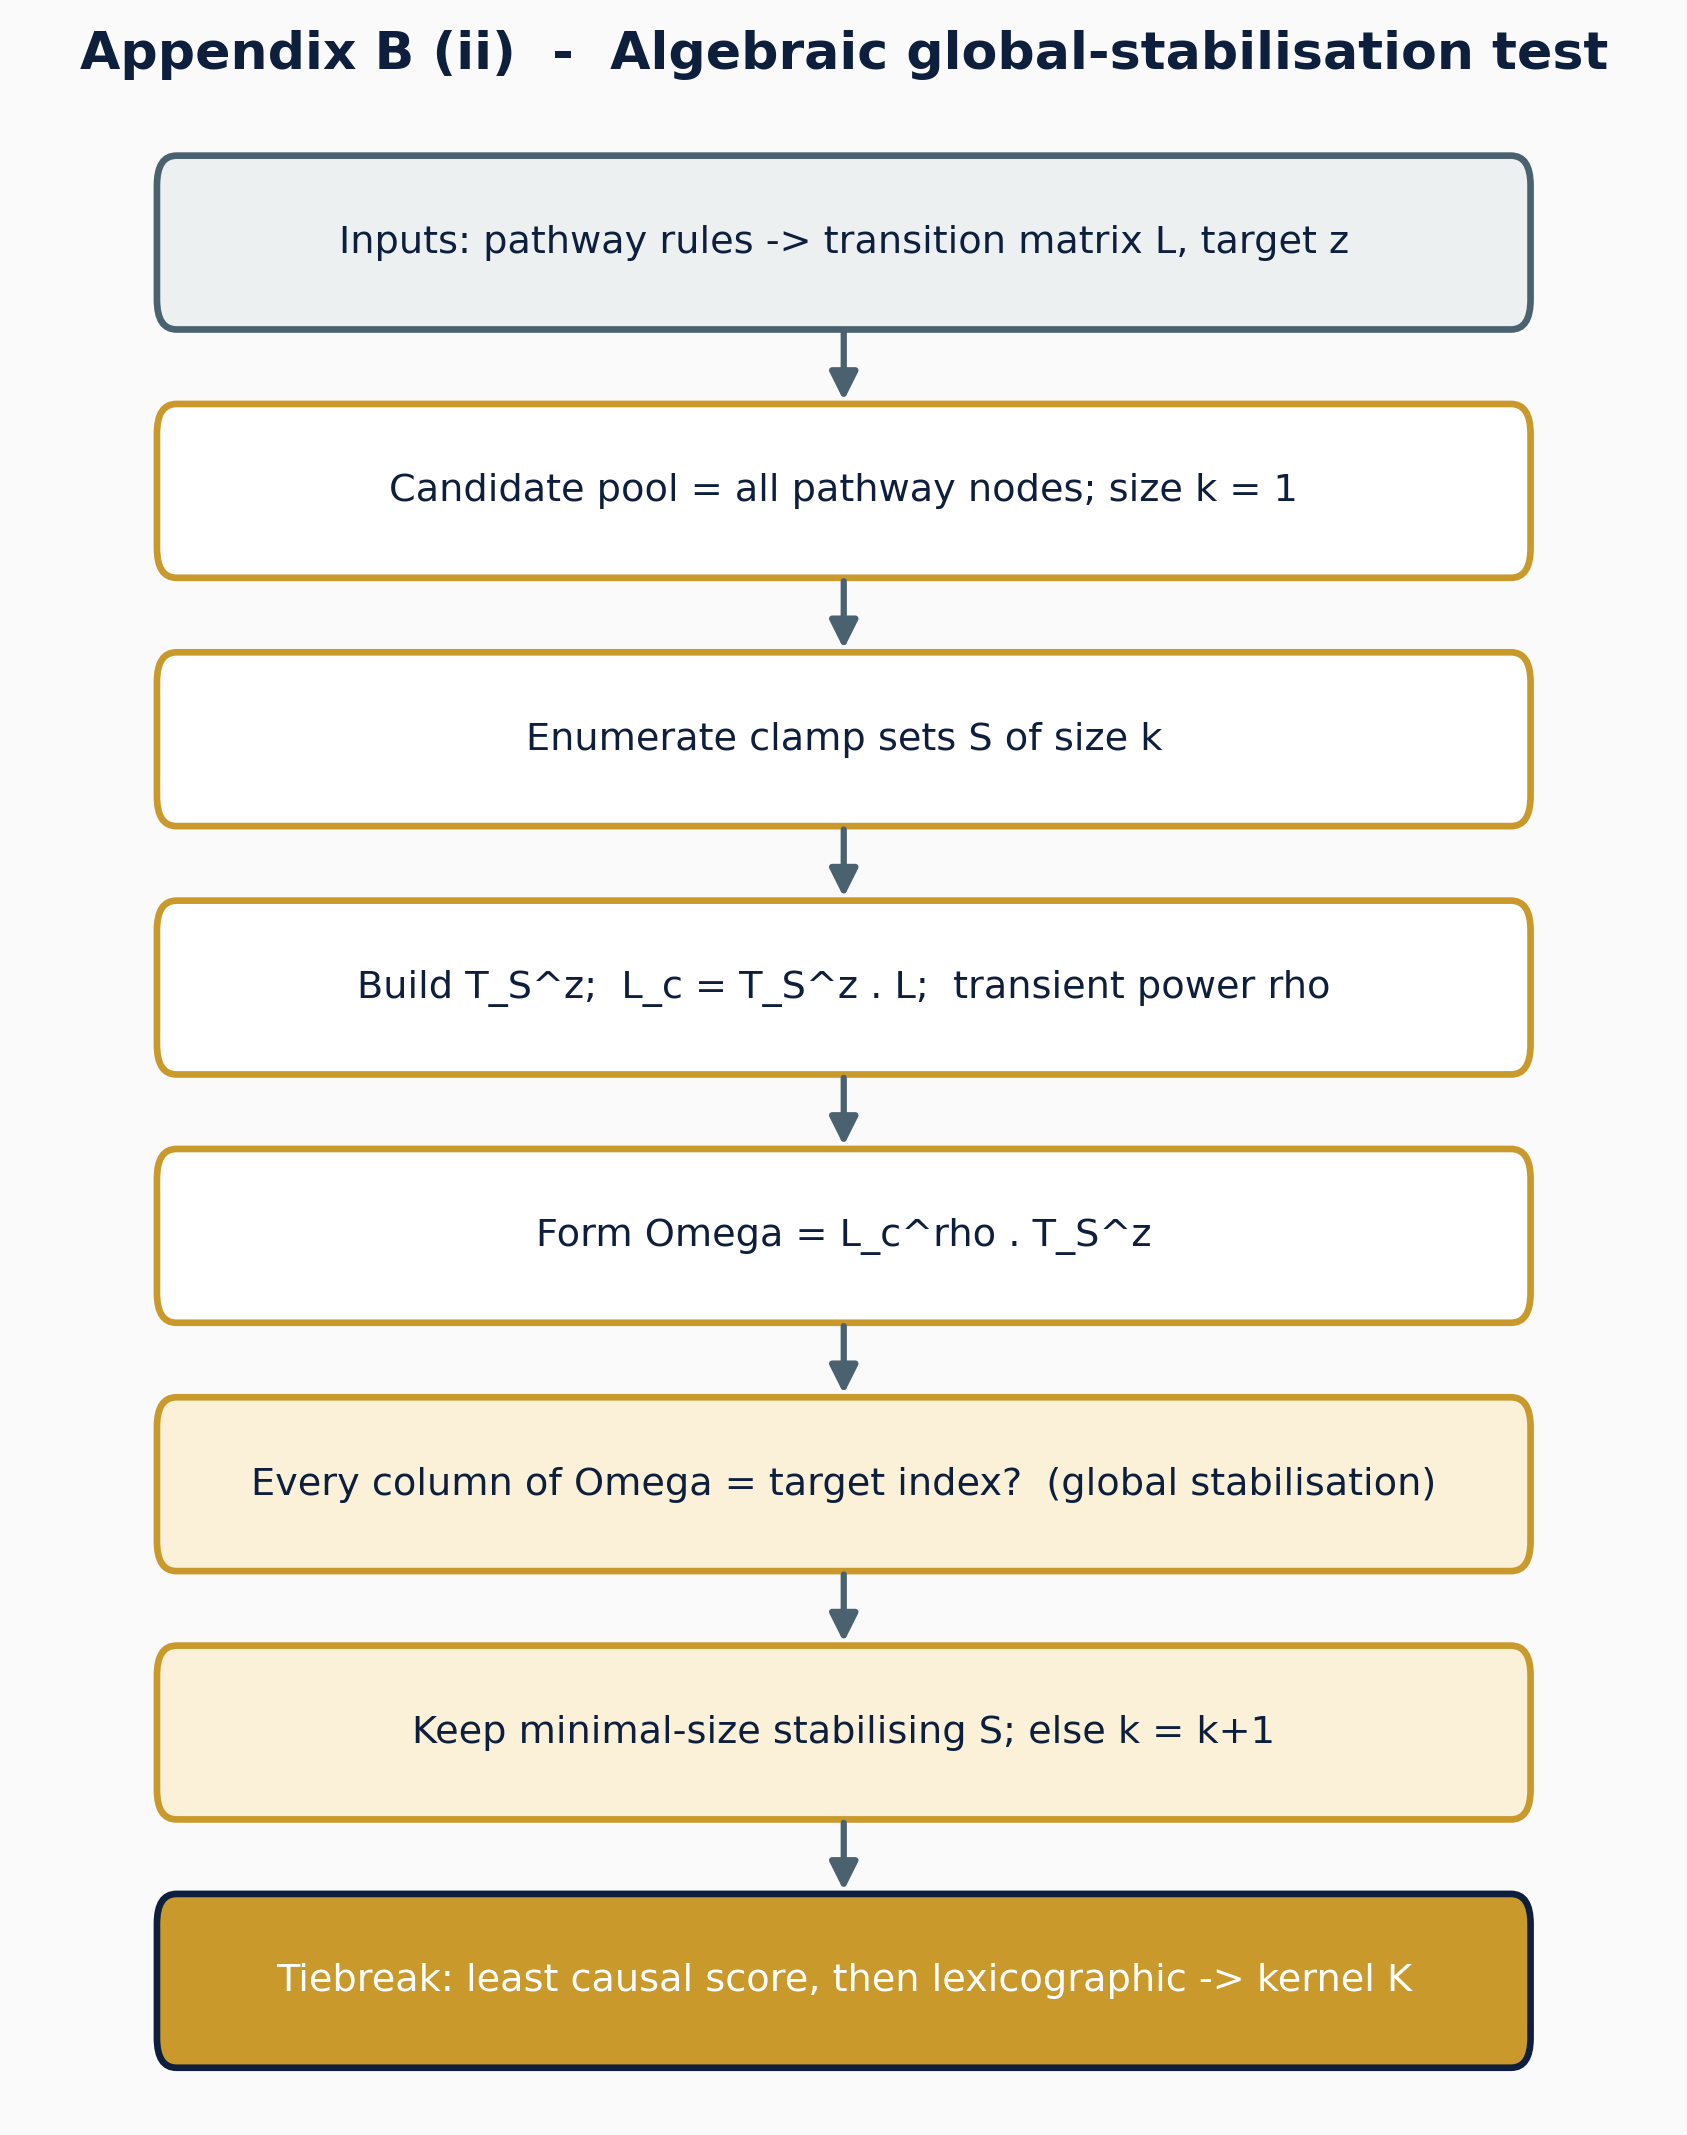
\includegraphics[width=0.6\textwidth]{figures/figC_flow_stabilize.png}
\caption{\textbf{Algebraic global-stabilisation test (Tier~1).} For each candidate clamp set $S$, the controlled operator $\Omega=L_c^{\rho}T_S^z$ is formed, and $S$ is accepted only if every column of $\Omega$ is the target index, that is, the clamp drives every pathway state to target, not only the patient's. Minimal-size accepted sets are kept and ties broken deterministically. This is the conservative, provable method used as the canonical kernel.}
\label{fig:flowstab}
\end{figure}

% Appendix C -- attributed restatement of the decomposition theorem of the prior preprint.
\section{The weak-coupling decomposition theorem (prior work)}
\label{app:theorem}

This appendix restates, for completeness, the pathway-decomposition theorem that the present
work positions itself against. The theorem and its proof are the contribution of the earlier
BBCN118 preprint~\cite{bhatti2026} (CC BY 4.0); the statement and proof sketch below are
reproduced and adapted from that work. They are included here so that the boundary identified
in Section~\ref{sec:32} can be read without consulting the source. The new content is the final
remark, which names the assumption the present network violates.

\paragraph{Setup.} Let a Boolean network with global update $x(t{+}1)=F(x(t))$ be partitioned into
$m$ pathway modules $P_1,\dots,P_m$, with module states $x_i$ and module targets $x_i^{*}$, so that
$x=(x_1,\dots,x_m)$ and $x^{*}=(x_1^{*},\dots,x_m^{*})$.

\paragraph{Theorem 1 (convergence under pathway decomposition).} Assume:
\begin{itemize}
\item[(A1)] \emph{Weak inter-pathway coupling:} $\displaystyle\max_{i\neq j}\left\|\partial F_i/\partial x_j\right\| < \varepsilon$, with $\varepsilon \ll 1$;
\item[(A2)] \emph{Local kernel effectiveness:} for each module $i$ there is a kernel $u_i$ that drives $x_i(t)\to x_i^{*}$ in finitely many steps; and
\item[(A3)] \emph{Modularity:} $F_i(x)\approx f_i\!\left(x_i, e_i(x)\right)$, where $e_i(x)$ collects the inputs $P_i$ receives from other modules.
\end{itemize}
Then the sequential application of the pathway kernels $u=\bigcup_{i=1}^{m} u_i$ drives the global
state into a neighbourhood of the target,
\[
x(t)\to \mathcal{N}_\delta(x^{*})=\{x : d_H(x,x^{*})\le \delta\},\qquad \delta = O(\varepsilon),
\]
where $d_H$ is the Hamming distance.

\paragraph{Proof sketch.} Take the weighted Hamming Lyapunov function
\[
V(x)=\sum_{i=1}^{m} w_i\, d_H\!\left(x_i,x_i^{*}\right),\qquad w_i>0 .
\]
$V$ is non-negative, integer-valued, bounded above by $\sum_i w_i|P_i|$, and zero exactly at $x^{*}$.
Intervening on module $k$ reduces its term by some $\alpha_k>0$ by (A2). By (A1) every other module
moves by at most $w_j\varepsilon|P_j|$, so
\[
\Delta V \le -\alpha_k + \varepsilon\sum_{j\neq k} w_j|P_j| ,
\]
which is strictly negative once $\varepsilon$ is small enough relative to $\alpha_k$. Because $V$ is
bounded below, strictly decreasing, and integer-valued, it reaches a minimum $V_{\min}$ in finitely
many steps, with $V_{\min}\le\delta=O(\varepsilon)$; at $\varepsilon=0$ the bound gives $V_{\min}=0$
and exact convergence. \hfill$\square$

\paragraph{Corollary 1 (convergence rate).} If each pathway kernel reduces the mismatch by at least
$\beta>0$ per intervention, the system reaches the neighbourhood in at most $T \le V(x(0))\,/\,(\beta/2)$
interventions.

\paragraph{Remark: why this paper is in the other regime.} The result holds only under assumption
(A1). The present BBCN network does not satisfy it. Its pathway-coupling graph carries a dominant
strongly-connected component of 16 of the 22 regulatory pathways (Section~\ref{sec:32}), so the
inter-module coupling is not small, the $O(\varepsilon)$ neighbourhood is not tight, and pathway-wise
stabilisation does not deliver joint reachability. That boundary is precisely what motivates modelling
the apoptosis core directly as the bistable switch of Setup~B. The full proof, including the explicit
$\varepsilon$ threshold, is given in the cited preprint and is not reproduced here.

% ------------------------------------------------------------
\begin{thebibliography}{99}
\bibitem{bhatti2026} Bhatti, A. I. From Pathway to Patient: Molecular Dysregulation as Basis for Minimal Sequential Intervention Strategy in Basal-Like Breast Cancer. \emph{Research Square} (2026). DOI: 10.21203/rs.3.rs-8942485/v1.
\bibitem{rafimanzelat2025} Rafimanzelat, M. R. Global stabilization of Boolean networks with applications to biomolecular network control. \emph{Sci. Rep.} \textbf{15}, 15201 (2025). DOI: 10.1038/s41598-025-97684-y.
\bibitem{zanudo2015} Za\~{n}udo, J. G. T. \& Albert, R. Cell fate reprogramming by control of intracellular network dynamics. \emph{PLoS Comput. Biol.} \textbf{11}(4), e1004193 (2015).
\bibitem{zanudo2013} Za\~{n}udo, J. G. T. \& Albert, R. An effective network reduction approach to find the dynamical repertoire of discrete dynamic networks. \emph{Chaos} \textbf{23}(2), 025111 (2013).
\bibitem{rozum2022} Rozum, J. C., Deritei, D., Park, K. H., Za\~{n}udo, J. G. T. \& Albert, R. pystablemotifs: Python library for attractor identification and control in Boolean networks. \emph{Bioinformatics} \textbf{38}, 1465--1466 (2022).
\bibitem{cheng2009} Cheng, D. \& Qi, H. Controllability and observability of Boolean control networks. \emph{Automatica} \textbf{45}, 1659--1667 (2009).
\bibitem{montagud2022} Montagud, A. et al. Patient-specific Boolean models of signalling networks guide personalised treatments. \emph{eLife} \textbf{11}, e72626 (2022).
\bibitem{beal2019} B\'{e}al, J., Montagud, A., Traynard, P., Barillot, E. \& Calzone, L. Personalization of logical models with multi-omics data allows clinical stratification of patients. \emph{Front. Physiol.} \textbf{9}, 1965 (2019).
\bibitem{wee2009} Wee, K. B. \& Aguda, B. D. Akt versus p53 in a network of oncogenes and tumour-suppressor genes regulating cell survival and death. \emph{PLoS ONE} \textbf{4}, e4407 (2009).
\bibitem{gao2005} Gao, T., Furnari, F. \& Newton, A. C. PHLPP: a phosphatase that directly dephosphorylates Akt. \emph{Mol. Cell} \textbf{18}, 13--24 (2005).
\bibitem{tarjan1972} Tarjan, R. Depth-first search and linear graph algorithms. \emph{SIAM J. Comput.} \textbf{1}, 146--160 (1972).
\bibitem{tcga2012} The Cancer Genome Atlas Network. Comprehensive molecular portraits of human breast tumours. \emph{Nature} \textbf{490}, 61--70 (2012).
\bibitem{metabric2012} Curtis, C. et al. The genomic and transcriptomic architecture of breast tumours (METABRIC). \emph{Nature} \textbf{486}, 346--352 (2012).
\bibitem{kauffman1969} Kauffman, S. A. Metabolic stability and epigenesis in randomly constructed genetic nets. \emph{J. Theor. Biol.} \textbf{22}, 437--467 (1969).
\bibitem{thomas1991} Thomas, R. Regulatory networks seen as asynchronous automata: a logical description. \emph{J. Theor. Biol.} \textbf{153}, 1--23 (1991).
\bibitem{albert2003} Albert, R. \& Othmer, H. G. The topology of the regulatory interactions predicts the expression pattern of the segment polarity genes in \emph{Drosophila melanogaster}. \emph{J. Theor. Biol.} \textbf{223}, 1--18 (2003).
\bibitem{saez2009} Saez-Rodriguez, J. et al. Discrete logic modelling as a means to link protein signalling networks with functional analysis of mammalian signal transduction. \emph{Mol. Syst. Biol.} \textbf{5}, 331 (2009).
\bibitem{morris2010} Morris, M. K., Saez-Rodriguez, J., Sorger, P. K. \& Lauffenburger, D. A. Logic-based models for the analysis of cell signaling networks. \emph{Biochemistry} \textbf{49}, 3216--3224 (2010).
\bibitem{helikar2012} Helikar, T. et al. The Cell Collective: toward an open and collaborative approach to systems biology. \emph{BMC Syst. Biol.} \textbf{6}, 96 (2012).
\bibitem{naldi2018} Naldi, A. et al. Logical modeling and analysis of cellular regulatory networks with GINsim 3.0. \emph{Front. Physiol.} \textbf{9}, 646 (2018).
\bibitem{fumia2013} Fumia, H. F. \& Martins, M. L. Boolean network model for cancer pathways: predicting carcinogenesis and targeted therapy outcomes. \emph{PLoS ONE} \textbf{8}, e69008 (2013).
\bibitem{vonderheyde2014} von der Heyde, S. et al. Boolean ErbB network reconstructions and perturbation simulations reveal individual drug response in different breast cancer cell lines. \emph{BMC Syst. Biol.} \textbf{8}, 75 (2014).
\bibitem{sgariglia2024} Sgariglia, D. et al. Optimizing therapeutic targets for breast cancer using Boolean network models. \emph{Comput. Biol. Chem.} \textbf{109}, 108022 (2024).
\bibitem{taoma2024} Taoma, K., Ruengjitchatchawalya, M., Liangruksa, M. \& Laomettachit, T. Boolean modeling of breast cancer signaling pathways uncovers mechanisms of drug synergy. \emph{PLoS ONE} \textbf{19}, e0298788 (2024).
\bibitem{zanudo2017} Gomez Tejeda Za\~{n}udo, J., Scaltriti, M. \& Albert, R. A network modeling approach to elucidate drug resistance mechanisms and predict combinatorial drug treatments in breast cancer. \emph{Cancer Converg.} \textbf{1}, 5 (2017).
\bibitem{fiedler2013} Fiedler, B., Mochizuki, A., Kurosawa, G. \& Saito, D. Dynamics and control at feedback vertex sets I: informative and determining nodes in regulatory networks. \emph{J. Dyn. Differ. Equ.} \textbf{25}, 563--604 (2013).
\bibitem{shmulevich2002} Shmulevich, I., Dougherty, E. R., Kim, S. \& Zhang, W. Probabilistic Boolean networks: a rule-based uncertainty model for gene regulatory networks. \emph{Bioinformatics} \textbf{18}, 261--274 (2002).
\bibitem{bhatti_arxiv2026} Bhatti, A. I. Pathway-Wise Sequential Control of Boolean Cancer Networks Reveals Structural Limits of Therapeutic Intervention. \emph{arXiv preprint} (2026).
\bibitem{brognard2007} Brognard, J., Sierecki, E., Gao, T. \& Newton, A. C. PHLPP and a second isoform, PHLPP2, differentially attenuate the amplitude of Akt signaling. \emph{Mol. Cell} \textbf{25}, 917--931 (2007).
\bibitem{chandarlapaty2011} Chandarlapaty, S. et al. AKT inhibition relieves feedback suppression of receptor tyrosine kinase expression and activity. \emph{Cancer Cell} \textbf{19}, 58--71 (2011).
\bibitem{turner2023} Turner, N. C. et al. Capivasertib in hormone receptor-positive advanced breast cancer (CAPItello-291). \emph{N. Engl. J. Med.} \textbf{388}, 2058--2070 (2023).
\bibitem{eissing2004} Eissing, T. et al. Bistability analyses of a caspase activation model for receptor-induced apoptosis. \emph{J. Biol. Chem.} \textbf{279}, 36892--36897 (2004).
\bibitem{legewie2006} Legewie, S., Bl\"{u}thgen, N. \& Herzel, H. Mathematical modeling identifies inhibitors of apoptosis as mediators of positive feedback and bistability. \emph{PLoS Comput. Biol.} \textbf{2}, e120 (2006).
\bibitem{bagci2006} Bagci, E. Z. et al. Bistability in apoptosis: roles of Bax, Bcl-2 and mitochondrial permeability transition pores. \emph{Biophys. J.} \textbf{90}, 1546--1559 (2006).
\bibitem{kimparkcho2013} Kim, J., Park, S.-M. \& Cho, K.-H. Discovery of a kernel for controlling biomolecular regulatory networks. \emph{Sci. Rep.} \textbf{3}, 2223 (2013).
\bibitem{albeck2008} Albeck, J. G. et al. Quantitative analysis of pathways controlling extrinsic apoptosis in single cells. \emph{Mol. Cell} \textbf{30}, 11--25 (2008).
\bibitem{lisun2011} Li, F. \& Sun, J. Controllability of Boolean control networks with time delays in states. \emph{Automatica} \textbf{47}, 603--607 (2011).
\bibitem{lu2016} Lu, J., Zhong, J., Ho, D. W. C., Tang, Y. \& Cao, J. On controllability of delayed Boolean control networks. \emph{SIAM J. Control Optim.} \textbf{54}, 475--494 (2016).
\bibitem{parmar2015} Parmar, K., Blyuss, K. B., Kyrychko, Y. N. \& Hogan, S. J. Time-delayed models of gene regulatory networks. \emph{Comput. Math. Methods Med.} \textbf{2015}, 347273 (2015).
\bibitem{brunet1999} Brunet, A. et al. Akt promotes cell survival by phosphorylating and inhibiting a Forkhead transcription factor. \emph{Cell} \textbf{96}, 857--868 (1999).
\bibitem{chen2010} Chen, J. et al. Constitutively nuclear FOXO3a localization predicts poor survival and promotes Akt phosphorylation in breast cancer. \emph{PLoS ONE} \textbf{5}, e12293 (2010).
\end{thebibliography}

\end{document}
